\chapter{Espace et géométrie} \label{Geo6}

% Grille
\newcommand{\cn}{\psframe[fillstyle=solid,fillcolor=black](0,0)(1,1)}
\newcommand{\ho}{\includegraphics[width=0.4cm]{Geometrie_did/Images/Geo6_analyse_Hercule_course}}
\newcommand{\po}{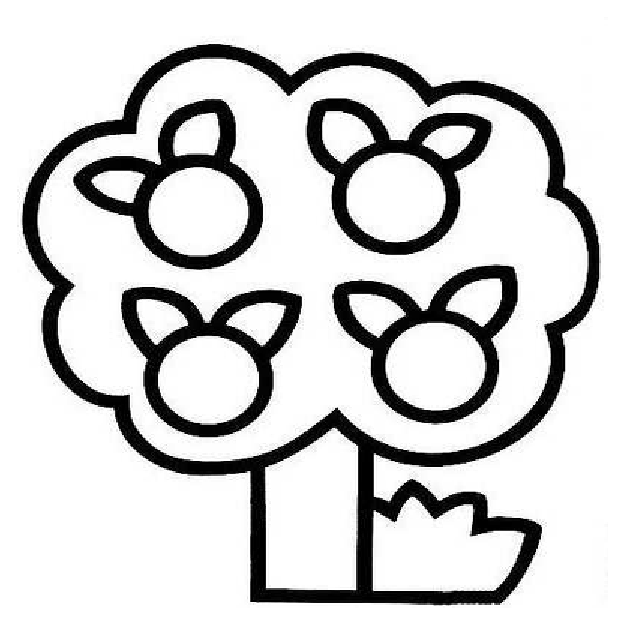
\includegraphics[width=0.4cm]{Geometrie_did/Images/Geo6_analyse_pommier}}

% Commandes
\newcommand{\dep}{\pspolygon[fillstyle=solid,fillcolor=orange](5.5,1)(0,1)(0,0)(1,0)(1.25,-0.25)(1.5,0)(6,0)(6,0.5) \pswedge[fillstyle=solid,fillcolor=orange,linecolor=orange](5.5,0.5){0.5}{0}{90} \psarc(5.5,0.5){0.5}{0}{90} \put(0.5,0.3){\footnotesize Démarre}}
\newcommand{\av}[1]{\pspolygon[fillstyle=solid,fillcolor=green](0,0)(1,0)(1.25,-0.25)(1.5,0)(6,0)(6,1)(1.5,1)(1.25,0.75)(1,1)(0,1) \put(0.5,0.3){\footnotesize Avance de #1}}
\newcommand{\tg}{\pspolygon[fillstyle=solid,fillcolor=yellow](0,0)(1,0)(1.25,-0.25)(1.5,0)(6,0)(6,1)(1.5,1)(1.25,0.75)(1,1)(0,1) \put(0.5,0.3){\footnotesize Tourne à gauche}}
\newcommand{\td}{\pspolygon[fillstyle=solid,fillcolor=pink](0,0)(1,0)(1.25,-0.25)(1.5,0)(6,0)(6,1)(1.5,1)(1.25,0.75)(1,1)(0,1) \put(0.5,0.3){\footnotesize Tourne à droite}}
\newcommand{\fin}{\pspolygon[fillstyle=solid,fillcolor=orange](0,0)(5.5,0)(6,0.5)(6,1)(1.5,1)(1.25,0.75)(1,1)(0,1)(0,0) \pswedge[fillstyle=solid,fillcolor=orange,linecolor=orange](5.5,0.5){0.5}{-90}{0} \psarc(5.5,0.5){0.5}{-90}{0} \put(0.5,0.3){\footnotesize Prends les pommes}}
\newcommand{\ret}[1]{\pspolygon[fillstyle=solid,fillcolor=blue!30](0,0)(1,0)(1.25,-0.25)(1.5,0)(6,0)(6,0.5)(2.5,0.5)(2.25,0.25)(2,0.5)(1,0.5)(1,2.5)(2,2.5)(2.25,2.25)(2.5,2.5)(6,2.5)(6,3.5)(1.5,3.5)(1.25,3.25)(1,3.5)(0,3.5) \put(0.5,2.8){\footnotesize Répète #1 fois}}
\newcommand{\reo}[1]{\pspolygon[fillstyle=solid,fillcolor=blue!30](0,0)(1,0)(1.25,-0.25)(1.5,0)(6,0)(6,0.5)(2.5,0.5)(2.25,0.25)(2,0.5)(1,0.5)(1,1.5)(2,1.5)(2.25,1.25)(2.5,1.5)(6,1.5)(6,2.5)(1.5,2.5)(1.25,2.25)(1,2.5)(0,2.5) \put(0.5,1.8){\footnotesize Répète #1 fois}}


\begin{prerequis}[Dans les programmes - cycle 1]
{\small
{\bf Se repérer dans le temps et dans l'espace}
   \begin{itemize}
      \item Situer des objets par rapport à soi, entre eux, par rapport à des objets repères.
      \item Se situer par rapport à d’autres, par rapport à des objets repères.
      \item Dans un environnement bien connu, réaliser un trajet, un parcours à partir de sa représentation (dessin ou codage).
      \item Élaborer des premiers essais de représentation plane, communicables (construction d’un code commun).
      \item Utiliser des marqueurs spatiaux adaptés (devant, derrière, droite, gauche, dessus, dessous\dots).
   \end{itemize}
{\bf Explorer des formes}
   \begin{itemize}
      \item Classer des objets en fonction de leur forme.
      \item Reconnaître quelques solides (cube, pyramide, boule, cylindre).
      \item Reproduire un assemblage de solides à partir d’un modèle.
   \end{itemize}}
\end{prerequis}

\begin{prerequis}[Dans les programmes - cycle 2]
{\small
{\bf (Se) repérer et (se) déplacer en utilisant des représentations}
   \begin{itemize}
      \item Se repérer dans son environnement proche.
      \item Situer des objets ou des personnes les uns par rapport aux autres ou par rapport à d’autres repères : vocabulaire des positions et des déplacements (gauche, droite, au-dessus, en dessous, sur, sous, devant, derrière, près, loin, nord, sud, est, ouest, avancer, reculer, tourner à droite/gauche, monter, descendre\dots).
      \item Produire des représentations des espaces familiers (école, quartier) et moins familiers : quelques modes de représentation de l’espace (maquettes, plans, photos).
      \item S’orienter et se déplacer en utilisant des repères.
      \item Réaliser des déplacements dans l’espace et les coder pour qu’un autre élève puisse les reproduire.
      \item Programmer les déplacements d’un robot ou d’un personnage sur un écran : repères spatiaux ; relations entre l’espace dans lequel on se déplace et ses représentations.
   \end{itemize}
{\bf Reconnaitre, nommer, décrire, reproduire quelques solides}
   \begin{itemize}
      \item Reconnaitre et trier les solides usuels parmi des solides variés.
      \item Reconnaître des solides simples dans son environnement proche.
      \item Réaliser et reproduire des assemblages de cubes et pavés droits les associer à des représentations (photos, vues\dots).
      \item Fabriquer un cube à partir d’un patron fourni : vocabulaire des solides (cube, pavé droit, boule, cylindre, cône, pyramide) et des polyèdres (face, sommet, arête) ; les faces d’un cube sont des carrés ; les faces d’un pavé droit sont des rectangles (qui peuvent être des carrés).
   \end{itemize}}
\end{prerequis}

\begin{prerequis}[Dans les programmes - cycle 3]
{\small
{\bf (Se) repérer et (se) déplacer dans l’espace en utilisant ou en élaborant des représentations}
   \begin{itemize}
      \item Se repérer, décrire ou exécuter des déplacements, sur un plan ou sur une carte (école, quartier, ville, village).
      \item Accomplir, décrire, coder des déplacements dans des espaces familiers.
      \item Programmer les déplacements d’un robot/personnage à l'écran en utilisant un logiciel de programmation : vocabulaire des positions et des déplacements (tourner à gauche/droite, $\frac12$ tour, $\frac14$ de tour).
      \item Diverses représentation de l’espace : maquettes, plans, schémas.
   \end{itemize}
{\bf Reconnaitre, nommer, décrire, reproduire, représenter, construire quelques solides}
   \begin{itemize}
      \item Reconnaitre, nommer, décrire des solides simples ou des assemblages de solides simples : cube, pavé droit, prisme droit, pyramide, cylindre, cône, boule. Vocabulaire associé à ces objets : hauteur solide, sommet, face, arête.
      \item Reproduire, représenter, construire des solides simples ou des assemblages de solides simples sous forme de maquettes ou de dessins ou à partir d’un patron (donné, dans le cas d’un prisme ou d’une pyramide, ou à construire dans le cas d’un pavé droit).
   \end{itemize}}
\end{prerequis}


%%%%%%%%%%%%%%%%%%%%
%%%%%%%%%%%%%%%%%%%%
\reperes


%%%%%%%%%%%%%%%%
\section{De repérer, se déplacer}
%%%%%%%%%%%%%%%%

%%%%%%%%%%%%%%%%%%%%%%%%%%
\subsection{Repérage dans l'espace en maternelle}
%%%%%%%%%%%%%%%%%%%%%%%%%%

Dans les programmes de 2018 [edu1] : \og par l’utilisation et la production de représentations diverses (photos, maquettes, dessins, plans, etc.) et également par les échanges langagiers avec leurs camarades et les adultes, les enfants apprennent à restituer leurs déplacements et à en effectuer à partir de consignes orales comprises et mémorisées. Ils établissent alors les relations entre leurs déplacements et les représentations de ceux-ci. Le passage aux représentations planes par le biais du dessin les amène à commencer à mettre intuitivement en relation des perceptions en trois dimensions et des codages en deux dimensions faisant appel à certaines formes géométriques (rectangles, carrés, triangles, cercles). Ces mises en relations seront plus précisément étudiées à l’école élémentaire, mais elles peuvent déjà être utilisées pour coder des déplacements ou des représentations spatiales. De plus, les dessins, comme les textes présentés sur des pages ou les productions graphiques, initient les enfants à se repérer et à s’orienter dans un espace à deux dimensions, celui de la page mais aussi celui des cahiers et des livres. \fg. \\

{\bf\large Faire l'expérience de l'espace}

On choisit des activités pour apprendre à effectuer des repérages dans l'espace réel (essentiellement dans le méso espace) permettent de : \\
 -- situer des objets par rapport à soi, le centre du repère étant l'enfant lui même : \og devant moi, à ma gauche, derrière moi, à ma droite, à côté de moi\dots \fg ; \\
 -- se situer par rapport à des objet, le centre de repère étant l’objet : \og je suis devant, je suis à côté, je sui loin\dots \fg ; \\
 -- situer des objets les uns par rapport aux autres, où le centre du repère peut varier \og en haut, en bas, à droite de, à gauche de, en dessous de \dots \fg \\
 -- se repérer lorsqu'on se déplace, ou le centre du repère est l'élève, qui bouge dans son espace.

{\renewcommand{\StringDOCUMENTATION}{Exemples de situations}
\begin{documentation}
\begin{itemize}
   \item Repérer les différents espaces de la classe puis de l'école \og où est la mascotte de la classe ? \fg
   \item Mettre l'élève en situation de se déplacer dans l'école, d'en explorer les lieux : aller à la cantine, à la BCD, aux toilette.
   \item Réaliser des parcours en salle de motricité.
   \item Jeux de Jacques a dit, chasse au trésor, kim visuel, placer des personnages. \\ [-7mm]
   \end{itemize}
\end{documentation}}

\medskip

{\bf\large Représenter l'espace}

On choisit des activités où on lit et on élabore des représentations de l’espace : maquettes, schémas, dessins\dots

{\renewcommand{\StringDOCUMENTATION}{Exemples de situations}
\begin{documentation}
   \begin{itemize}
      \item Manipuler des photos des différents lieux de l'école (classe, salle de jeux, cour). Décrire et apprendre à reconnaître et associer ces lieu à sa photo.
      \item  Réaliser une maquette, un plan, se servir d'un plan pour se déplacer)
      \item Observer des objets suivant des vues différentes, les représenter.
      \item Jeux d'organisation spatiale dans le micro-espace : reproduire, coder, observer, prendre en compte des contraintes, créer un assemblage de solides. \\ [-7mm]
   \end{itemize}
\end{documentation}}

\smallskip

\pagebreak


\subsection{Repérage et codage} %%%

\smallskip

{\bf\large Pourquoi enseigner le code à l'école ?}

D'après le document {\it Proposition d'orientations générales pour un programme d'informatique à l'école primaire} [abi13] : \og L'école primaire doit être le temps de la découverte des concepts fondamentaux de l'informatique, celui où l'on parle aux élèves, avec leurs mots, à partir de leur quotidien et de leurs connaissances acquises dans les autres disciplines, d'informations, de langages de programmation, d'algorithmes et de machines. L'enseignement de l'informatique à l'école nous semble être trop souvent limité à l'utilisation d'ordinateurs et de logiciels créés par d'autres. Cette vision dénature une discipline scientifique et technique qui donne un rôle essentiel à l'abstraction et à l'expérimentation personnelle. Faire de l'informatique ne consiste pas à passer des heures devant un écran, mais à acquérir des notions fondamentales et universelles. L'initiation à l'informatique doit donc n'être liée ni à un ordinateur particulier, ni à un logiciel particulier, ni à un langage particulier. Elle doit par ailleurs chercher un équilibre entre des activités fondées sur l'utilisation d'un ordinateur et des activités débranchées, c'est-à-dire ne recourant pas à une telle utilisation. \fg \\
 
En effet, les élèves ont souvent une attitude consommatrice vis-à-vis de l'informatique : on allume, on choisit un logiciel ou une application, puis on applique \og bêtement \fg{}. L'idée du code à l'école serait de profiter de l'utilisation de cet outil pour s'interroger sur son fonctionnement, pour lui donner du sens, pour le critiquer, et de cette interrogation pourrait naître l'occasion d'échanges collectifs. L'initiation à l'informatique doit aussi passer par la découverte des concepts fondamentaux de langage et d'algorithmes, sans toujours utiliser un ordinateur pour cela. \\
Voici une illustration de {\it Brian Aspinall}, traduite par {\it François Bocquet} qui résume les avantages du code et de la programmation à l'école :
\begin{center}
   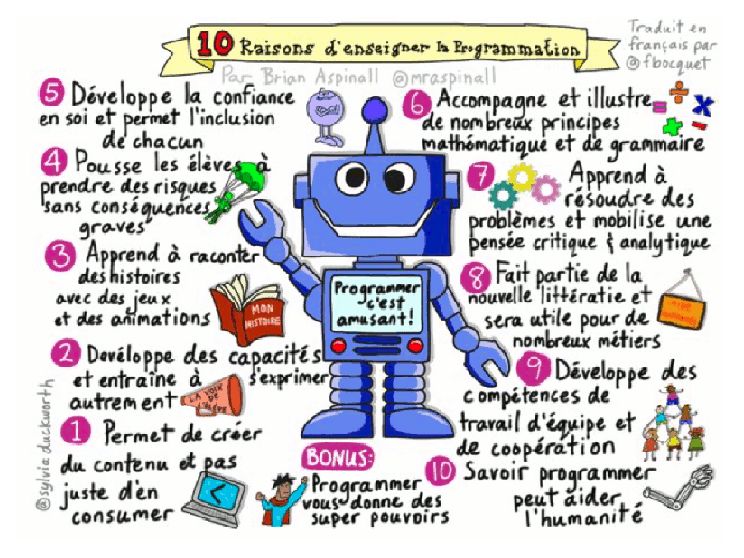
\includegraphics[width=14cm]{Geometrie_did/Images/Geo6_cours_pourquoi_coder_ecole}
\end{center}

\pagebreak


{\bf\large Deux langages de déplacement} \smallskip %%%

Le langage est la capacité de communiquer au moyen d'un système de signes (vocaux, gestuels, graphiques\dots) doté notamment d'un vocabulaire (les mots pour l'exprimer) et d'une grammaire (la syntaxe) [dow].

Une large part des nouveaux programmes concernant le code demande de programmer le déplacement d'un robot ou d'un personnage sur un quadrillage ou sur un écran. Pour cela, nous allons voir deux exemples de langages formels distincts qui peuvent paraître proches, mais qui en réalité ne font pas appel aux mêmes capacités de représentation de l'espace.

{\renewcommand{\StringDOCUMENTATION}{Deux langages bien distincts}
\begin{documentation}
\begin{itemize}
   \item le langage A composé des mots de vocabulaire : \og haut \fg{}, \og bas \fg{}, \og droite \fg{} et \og gauche \fg ;
   \item le langage R composé des mots de vocabulaire  \og avancer \fg{}, \og tourner à droite \fg{} (qui signifie \og tourner sur soi-même d'un quart de tour vers la droite \fg) et \og tourner à gauche \fg. \\ [-7mm]
\end{itemize}
\end{documentation}}

\medskip

Supposons, par exemple, que l'on souhaite coder le déplacement du quadrillage suivant :

\begin{minipage}{6cm}
   {\psset{unit=0.7}
   \begin{pspicture}(-4,-1.5)(4,4.7)
      \psgrid[subgriddiv=1,gridlabels=0mm](0,-1)(5,4)
      \psdots[linecolor=B2,linewidth=1mm](0.5,0.5)(3.5,2.5)     
      \psline[linecolor=B2,arrowsize=3mm]{->}(0.5,0.5)(1,0.5)
      \psline[linecolor=B2,arrowsize=3mm]{->}(0.5,0.5)(2.5,0.5)(2.5,2.5)(3.5,2.5)
   \end{pspicture}}
\end{minipage}
\qquad
\begin{minipage}{4cm}
   Avec le langage A : \\
   {\it droite - droite - haut - haut - droite} \\
   \ \\
\end{minipage}
\qquad
\begin{minipage}{4cm}   
   Avec le langage R : \\
   {\it avancer - avancer - tourner à gauche - avancer - avancer - tourner à droite - avancer} \\
\end{minipage}

Hormis le fait que le nombre d'instructions est supérieur dans le langage R, une autre différence très importante du point de vue de la structuration apparait ici : pour le langage A, le déplacement se fait comme si on se plaçait depuis l'extérieur du quadrillage, par exemple avec une vue du dessus. Ce repérage dépend donc de l'orientation de la feuille, indépendamment du point de vue de l'observateur. Pour ces raisons, il est appelé repérage {\bf Absolu}. En revanche, pour le langage R, c'est un autre point de vue qui est adopté : on se met à la place de l'observateur et l'orientation du quadrillage n'a aucun effet sur le codage obtenu. Le repérage est qualifié de {\bf Relatif}.

On pourra alors étudier ces deux langages et les comparer : apprendre à traduire un itinéraire d’un langage dans un autre ; étudier les avantages et inconvénients de chaque langage ; étudier l'effet d'une \og erreur \fg{} ; comment améliorer l'ergonomie du code ; rechercher des propriétés\dots \\

À l'école élémentaire, les élèves apprennent à se déplacer à l'aide d'un quadrillage ou de n\oe uds : en premier lieu, ils doivent repérer des cases ou des noeuds  d'un quadrillage grâce à un repérage absolu (souvent un couple de coordonnées : une lettre et un chiffre). Il n'y a pas lieu dans ce cas de se décentrer : on \og lit \fg{} directement les coordonnées de la case. L'exercice doit se faire dans les deux sens (codage et décodage).
\begin{center}
   {\psset{unit=0.65}
   \begin{pspicture}(-1,-0.3)(8,5.5)
      \rput(3.2,5){1) Ecris la position de chaque forme}
      \psgrid[subgriddiv=1,gridlabels=0](0,0)(4,4)
      \rput(-0.5,0.5){1}
      \rput(-0.5,1.5){2}
      \rput(-0.5,2.5){3}
      \rput(-0.5,3.5){4}
      \rput(0.5,-0.5){A}
      \rput(1.5,-0.5){B}
      \rput(2.5,-0.5){C}
      \rput(3.5,-0.5){D}
      \rput(0.5,3.5){\large$\diamondsuit$}
      \rput(1.5,2.5){\large$\spadesuit$}
      \rput(2.5,0.5){\large$\heartsuit$}
      \rput(3.5,1.5){\large$\clubsuit$}
      \rput(6,0.5){\large$\clubsuit$\,(\quad,\quad)} 
      \rput(6,1.5){\large$\spadesuit$\,(\quad,\quad)}  
      \rput(6,2.5){\large$\heartsuit$\,(\quad,\quad)} 
      \rput(6,3.5){\large$\diamondsuit$\,(\quad,\quad)} 
   \end{pspicture}
   \qquad
   \begin{pspicture}(-1,-0.3)(8,5.5)
      \rput(3.2,5){2) Dessine les formes sur le quadrillage}
      \psgrid[subgriddiv=1,gridlabels=0](0,0)(4,4)
      \rput(-0.5,0.5){1}
      \rput(-0.5,1.5){2}
      \rput(-0.5,2.5){3}
      \rput(-0.5,3.5){4}
      \rput(0.5,-0.5){A}
      \rput(1.5,-0.5){B}
      \rput(2.5,-0.5){C}
      \rput(3.5,-0.5){D}
      \rput(6,0.5){\large$\clubsuit$\,(\,C\,,\,3\,)} 
      \rput(6,1.5){\large$\spadesuit$\,(\,B\,,\,1\,)}  
      \rput(6,2.5){\large$\heartsuit$\,(\,A\,,\,4\,)}
      \rput(6,3.5){\large$\diamondsuit$\,(\,D\,,\,2\,)}
   \end{pspicture}}
\end{center}

Puis, l'élève apprend à se déplacer sur un quadrillage en codant les déplacements. 
\begin{center}
   {\psset{unit=0.45}
   \begin{pspicture}(0,0.2)(18,6.8)
      \psgrid[subgriddiv=1,gridlabels=0,gridcolor=gray](0,0)(7,7)
      \rput(1,1){\Large$\heartsuit$}
      \psline[linewidth=0.5mm]{->}(1,1)(2,1)
      \psline[linewidth=0.5mm]{->}(2,1)(2,2)
      \psline[linewidth=0.5mm]{->}(2,2)(3,2)
      \psline[linewidth=0.5mm]{->}(3,2)(3,3)
      \psline[linewidth=0.5mm]{->}(3,3)(4,3)
      \psline[linewidth=0.5mm]{->}(4,3)(5,3)
      \psline[linewidth=0.5mm]{->}(5,3)(5,2)
      \psline[linewidth=0.5mm]{->}(5,2)(6,2)
      \rput(6,2){\Large$\diamondsuit$}
      \rput(3,4){\Large$\spadesuit$}
      \psline[linewidth=0.5mm]{->}(3,4)(2,4)
      \psline[linewidth=0.5mm]{->}(2,4)(2,5)
      \psline[linewidth=0.5mm]{->}(2,5)(3,5)
      \psline[linewidth=0.5mm]{->}(3,5)(3,6)
      \psline[linewidth=0.5mm]{->}(3,6)(4,6)
      \psline[linewidth=0.5mm]{->}(4,6)(5,6)
      \psline[linewidth=0.5mm]{->}(5,6)(6,6)
      \psline[linewidth=0.5mm]{->}(6,6)(6,5)
      \rput(6,5){\Large$\clubsuit$}
      \psgrid[subgriddiv=1,gridlabels=0,gridcolor=gray](8,1)(18,2)
      \rput(8.5,1.5){\Large$\heartsuit$}
      \rput(9.5,1.5){$\rightarrow$}
      \rput(10.5,1.5){$\uparrow$}
      \rput(11.5,1.5){$\rightarrow$}
      \rput(12.5,1.5){$\uparrow$}
      \rput(13.5,1.5){$\rightarrow$}
      \rput(14.5,1.5){$\rightarrow$}
      \rput(15.5,1.5){$\downarrow$}
      \rput(16.5,1.5){$\rightarrow$}
      \rput(17.5,1.5){\Large$\diamondsuit$}
      \psgrid[subgriddiv=1,gridlabels=0,gridcolor=gray](8,4)(18,5)
      \rput(8.5,4.5){\Large$\spadesuit$}
      \rput(17.5,4.5){\Large$\clubsuit$}
      \rput(15,6.5){Ecris le message pour coder le déplacement}
   \end{pspicture}}
\end{center}
Nous sommes ici dans un déplacement fléché transposé dans un langage absolu plus \og visuel \fg. Le message peut être amélioré en remplaçant par exemple la suite \og $\rightarrow\,\rightarrow$ \fg{} par \og 2 $\rightarrow$ \fg, par exemple. \smallskip

Le langage relatif demande plus d'abstraction et l'élève doit se décentrer afin de se mettre à la place de l'objet que l'on veut faire bouger. C'est régulièrement ce type de langage qui est utilisé dans la robotique et la programmation car il ne dépend pas de l'endroit duquel on se place.
\begin{exemple*1}
Coder le déplacement de la voiture jusqu'au drapeau d'arrivée. La voiture se déplace selon les instructions qu'elle reçoit, comme un conducteur qui exécute les instructions données par son GPS. \\
\begin{minipage}{8cm}
   {\psset{unit=0.7}
   \begin{pspicture}(-1.5,0)(2.5,2)
      \psframe(0,0)(2.1,2)
      \psline[linewidth=2mm,arrowlength=1]{->}(1,0.3)(1,1.7)
   \end{pspicture}
   \begin{pspicture}(0,0)(2.5,2)
      \psframe(0,0)(2,2)
      \psline[linewidth=2mm,arrowlength=1]{->}(0.6,0.3)(0.6,1.4)(1.6,1.4)
   \end{pspicture}
   \begin{pspicture}(0,0)(2,2)
      \psframe(0,0)(2,2)
      \psline[linewidth=2.5mm,arrowlength=1]{->}(1.4,0.3)(1.4,1.4)(0.4,1.4)
   \end{pspicture}}
\end{minipage}
\qquad
\begin{minipage}{5cm}   
   {\psset{unit=0.5cm}
   \begin{pspicture}(0,0.5)(6,5.5)
      \psframe[fillstyle=solid,fillcolor=lightgray](1,1)(5,2)
      \psframe[fillstyle=solid,fillcolor=lightgray](5,2)(4,5)
      \psframe[fillstyle=solid,fillcolor=lightgray](2,4)(4,5)
      \psframe[fillstyle=solid,fillcolor=lightgray](0,3)(3,4)
      \psframe[fillstyle=solid,fillcolor=lightgray](0,4)(1,5)
      \psline(0.2,5.2)(0.2,5.8)(0.8,5.8)(0.8,5.5)(0.2,5.5)
      \psframe[fillstyle=solid,fillcolor=black](0.2,5.5)(0.35,5.65)
      \psframe[fillstyle=solid,fillcolor=black](0.35,5.65)(0.5,5.8)
      \psframe[fillstyle=solid,fillcolor=black](0.5,5.5)(0.65,5.65)
      \psframe[fillstyle=solid,fillcolor=black](0.65,5.65)(0.8,5.8)
      \psgrid[gridlabels=0,subgriddiv=1,gridcolor=gray](0,1)(6,6)
      \rput(0.5,1.5){
\includegraphics[width=5mm]{Geometrie_did/Images/Geo6_cours_F1}}
   \end{pspicture}} 
\end{minipage}
\end{exemple*1} 
\smallskip
Il est important de faire verbaliser les élèves sur la signification des flèches : la première flèche (avancer) correspond implicitement à une déplacement d'une case \og dans le sens de la voiture \fg. De la même manière, la deuxième flèche (tourner à droite) ne correspond pas à un déplacement latéral vers la droite, mais à un quart de tour vers la droite, sans toutefois changer de case. On observe ainsi une différence entre l'utilisation réelle de l'action \og tourner à droite \fg{} et son utilisation dans un algorithme : en effet, lorsqu'un élève est à pied ou à vélo et qu'il tourne à droite, cette action est associée à un déplacement en même temps qu'il tourne alors que, en programmation, elle correspond uniquement à une rotation tout en restant sur place. \smallskip


\subsection{Repères de progressivité à l'école élémentaire} %%%

\smallskip

{\bf\large Ce que disent les repères annuels}

-- {\bf Au CP}, les élèves représentent des lieux et codent des déplacements se situant dans la classe en mode débranché (papier/crayon, activité de motricité), puis dans l’environnement de l’école. \\
   Ils peuvent commencer à coder des déplacements à l’aide d’un logiciel de programmation adapté.

-- {\bf Au CE1 et CE2}, les élèves représentent des lieux et codent des déplacements se situant dans le quartier proche en mode débranché. Ils commencent, ou poursuivent le codage des déplacements à l’aide d’un logiciel au CE1, et consolident ces codage au CE2 : ils comprennent et produisent des algorithmes simples pour la programmation des déplacements d’un robot ou ceux d’un personnage sur un écran tout en  continuant à jouer physiquement ces situations dans l’espace concret.
   
-- {\bf Au CM1 et CM2}, les élèves apprennent à programmer le déplacement d’un personnage sur un écran : ils commencent par compléter de tels programmes, puis ils apprennent à corriger un programme erroné. Enfin, ils créent eux-mêmes des programmes (en absolu ou relatif) permettant d’obtenir des déplacements.

\pagebreak


{\bf\large Un exemple de progression} %%%

On adoptera une progression en travaillant d'abord dans le méso-espace afin que les élèves puissent appréhender cet espace pour passer progressivement de la manipulation de robots au travail dans le micro-espace.

{\psset{unit=0.95}
\begin{pspicture}(0,-0.2)(17,20.4)
   \rput(1,20){\bf méso}
   \rput(1,19.5){\bf espace}
   \psline[linewidth=1mm]{->}(1,19)(1,1)
   \rput(1,0.5){\bf micro}
   \rput(1,0){\bf espace}
   \rput(4,18){\bf Le robot idiot}
   \rput(4,17){\blue\small code}
   \rput(4,16.5){\blue\small algorithme}
   \rput(4,16){\blue\small programme}
   \rput(9,17.5){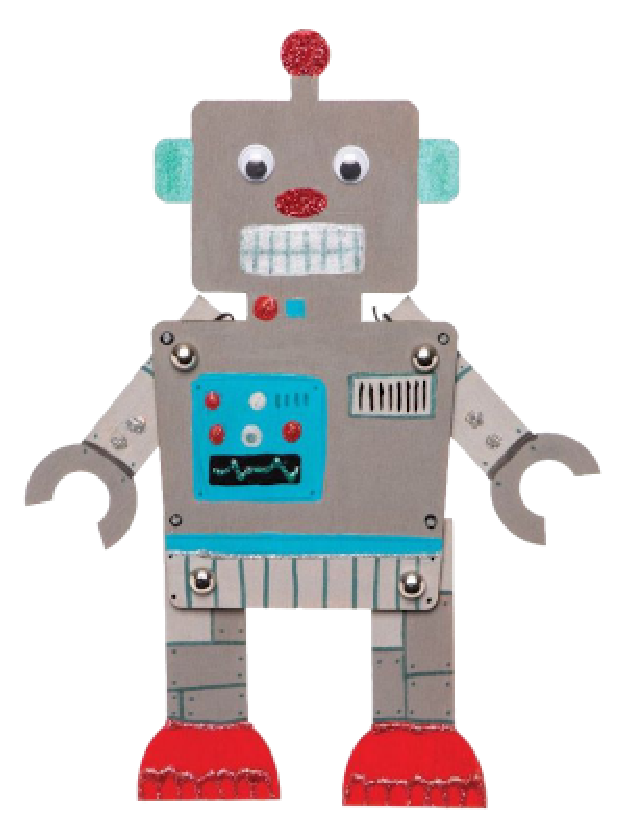
\includegraphics[width=3.3cm]{Geometrie_did/Images/Geo6_cours_robot}}
   \psline{<->}(13,18.5)(11,17.5)(13,16.5)
   \rput(15,19){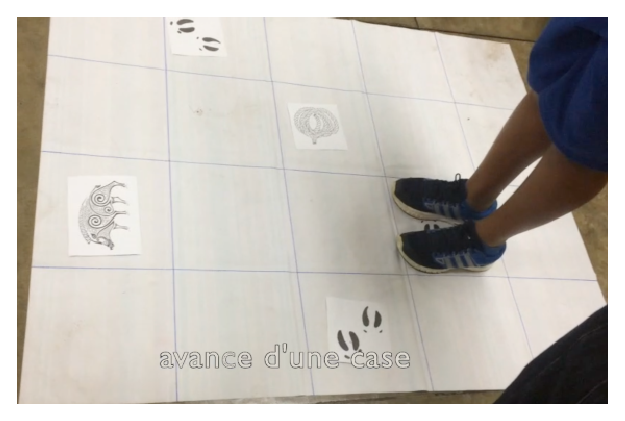
\includegraphics[width=3.5cm]{Geometrie_did/Images/Geo6_cours_robot_idiot_quadrillage}}
   \rput(15,16){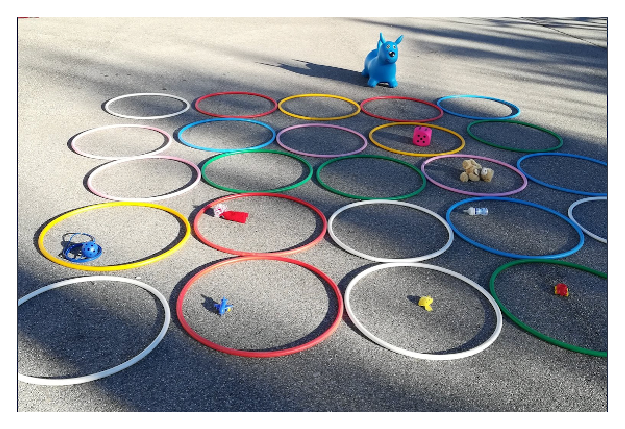
\includegraphics[width=3.5cm]{Geometrie_did/Images/Geo6_cours_robot_idiot_cerceaux}}
   \psline{->}(9,15)(9,13)
   \rput(4,12){\bf Manipulation de robots}
   \rput(4,10.5){\blue\small robot}
   \rput(4,11){\blue\small capteurs}
   \rput(4,10){\blue\small automate}
   \rput(9,11){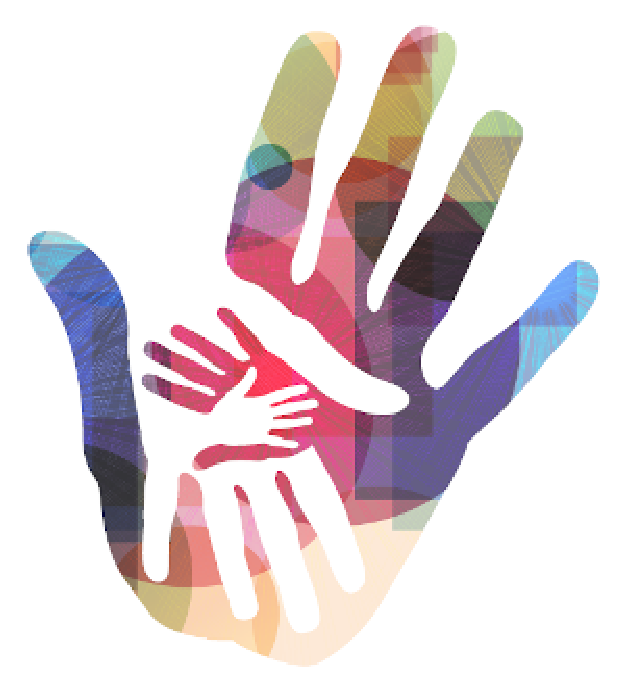
\includegraphics[width=3cm]{Geometrie_did/Images/Geo6_cours_manip}}
   \psline{<->}(12.5,11.5)(10.7,10.5)(12.5,9.5)
   \psline{->}(10.7,10.5)(12.5,10.5)
   \rput(14,12.5){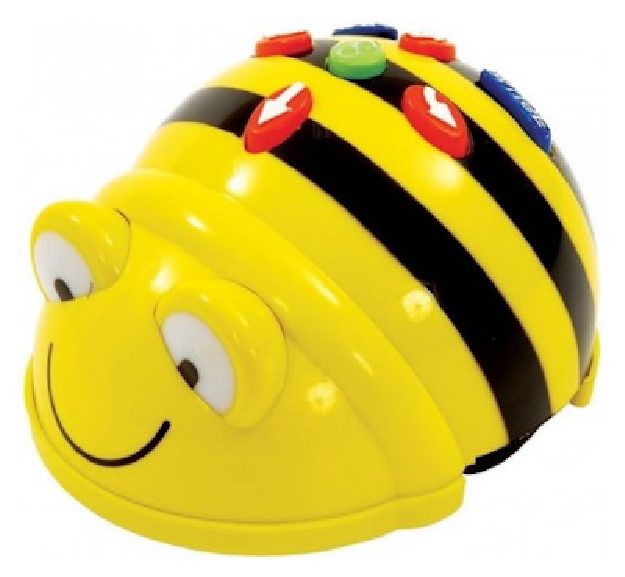
\includegraphics[width=2.2cm]{Geometrie_did/Images/Geo6_cours_beebot}}
   \rput(16,12.5){\blue\small beebot}
   \rput(16.5,10.5){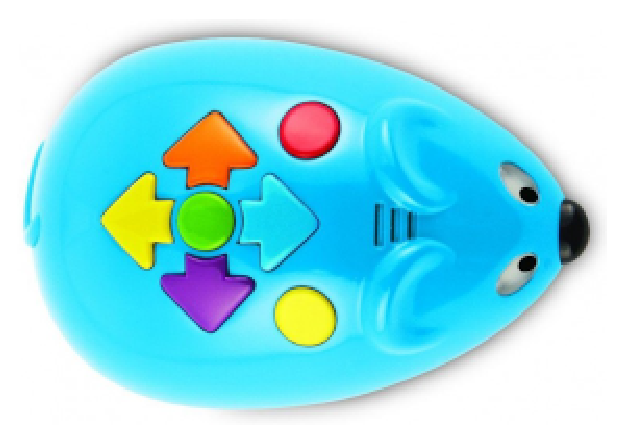
\includegraphics[width=2.5cm]{Geometrie_did/Images/Geo6_cours_robot_souris}}
   \rput(14,10.5){\blue\small robot souris}
   \rput(14,8.5){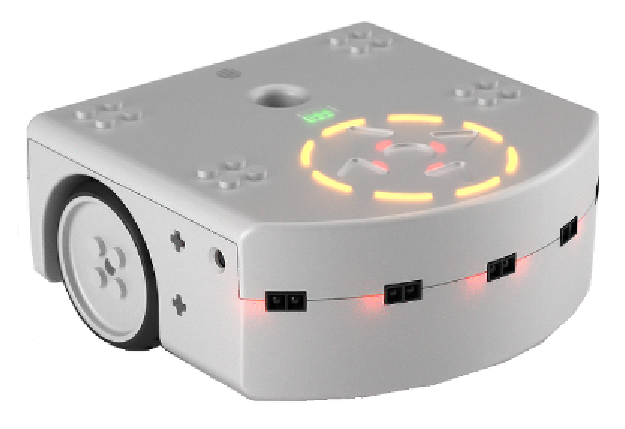
\includegraphics[width=2.5cm]{Geometrie_did/Images/Geo6_cours_thymio}}
   \rput(16.1,8.5){\blue\small thymio} 
   \psline{->}(9,7.5)(6,5)
   \rput(4,2.5){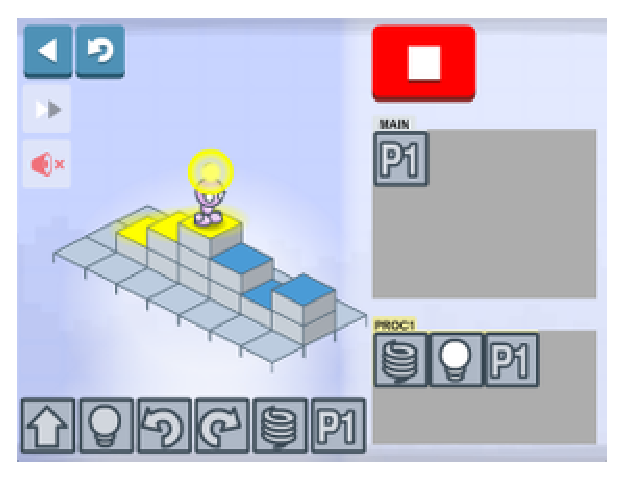
\includegraphics[width=4cm]{Geometrie_did/Images/Geo6_cours_lightbot}}
   \rput(4,4.5){\bf Logiciels}
   \psline{->}(9,9)(9,5)
   \rput(9,2.33){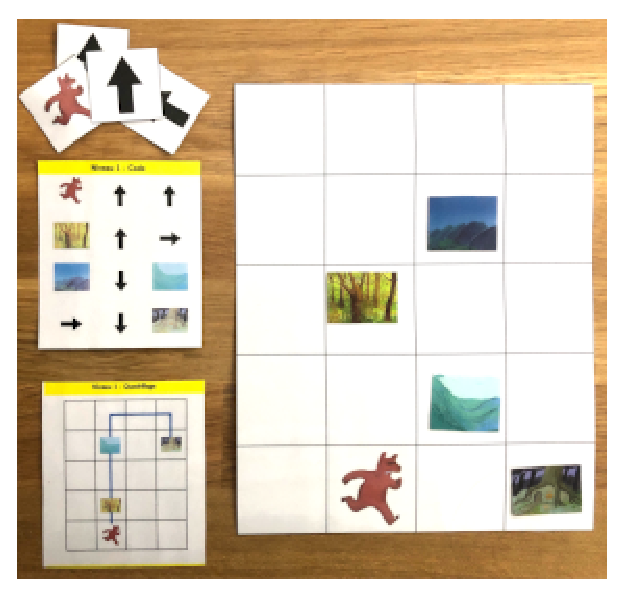
\includegraphics[width=3.5cm]{Geometrie_did/Images/Geo6_cours_cartacoder}}
   \rput(9,4.5){\bf Cartes}
   \psline{->}(9,7.5)(12,5)
   \rput(14,2.1){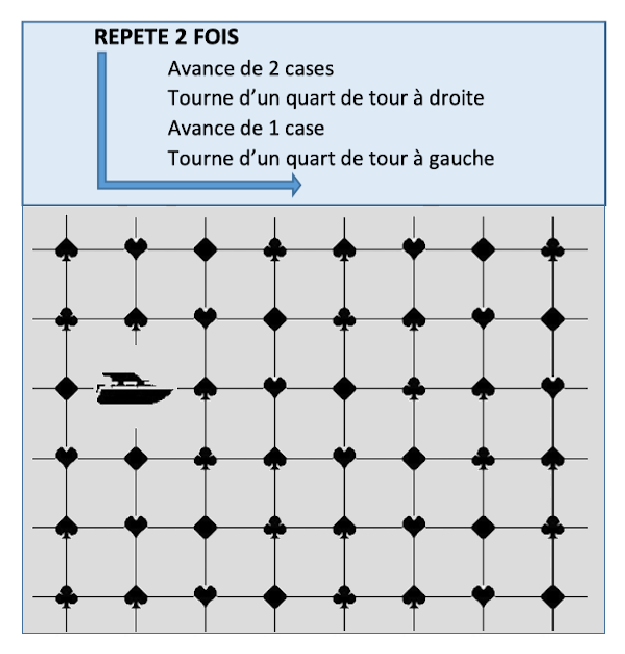
\includegraphics[width=3.7cm]{Geometrie_did/Images/Geo6_cours_bateau}}
   \rput(14,4.5){\bf Papier-crayon}
\end{pspicture}}

Le site [La main à la pâte] propose de nombreuses activités à faire faire aux élèves, du cycle 1 au cycle 4.


\subsection{Outils pour coder et programmer !} %%%

Passons de la théorie à la pratique avec une liste de ressources (non exhaustive !!!) qui permettent d'initier des enfants, même très jeunes, aux principes de la programmation et de la logique sous différentes formes.

%{\renewcommand{\StringDOCUMENTATION}{Des outils pour coder et programmer}
%\begin{documentation}
%\begin{itemize}
%   \item Diriger des {\bf robots} : il s'agit en général d'un petit robot que l'on peut programmer de façon simplifiée. Son inconvénient principal est qu'il est assez coûteux mais il est aussi très ludique et permet de voir concrètement l'effet d'un programme.
%   \item Des {\bf jeux de déplacement} : ils consistent à donner des instructions à un personnage à l'écran afin de le faire se déplacer selon des codes précis.
%   \item Des applications et logiciels de {\bf programmation} utilisant des {\bf blocs} logiques à assembler, choisis parmi une liste. Certains nécessitent de savoir lire, d'autre non car ils comportent un pictogramme représentant l'action à effectuer dessus.
%   \item Des {\bf sites Internet} dédiés à l'apprentissage du  code dès le plus jeune âge.
%   \item Des activités {\bf déconnectées}, utilisant ni ordinateur, ni  tablette, ni smartphone. \\ [-7mm]
%\end{itemize}
%\end{documentation}}

{\hautab{1.2}
\begin{Ltableau}{\linewidth}{2}{C{1.8}|p{14.15cm}}
   \hline
   \multicolumn{2}{|c|}{Les jeux débranchés} \\
   \hline
   \href{https://cutt.ly/kLQNT3a}{\blue Robot-idiot}
   &
   Le \og robot-idiot \fg{} doit sortir d’un labyrinthe que l’on aura construit sur une nappe, à l'aide de cerceaux, ou en dessinant à la craie sur le sol de la cour. Grâce à des instructions simples, il s'agit de faire sortir le robot du labyrinthe. Prix : gratuit. C1-C3. \\
   \hline
   \href{https://code.org/files/CSEDrobotics.pdf}{\blue My robotic} \href{https://code.org/files/CSEDrobotics.pdf}{\blue Friends}
   &
   Il s'agit de donner des instructions afin de construire une pyramide avec des gobelets, à l'aide d'un code fléché à écrire sur une feuille de papier. Prix : gratuit. C2-C3. \\
   \hline
\end{Ltableau}


\begin{Ltableau}{\linewidth}{2}{C{1.8}|p{14.15cm}}
   \hline
   \multicolumn{2}{|c|}{Les robots} \\
   \hline
   Bee-bot blue-bot
   &
   Abeille motorisée, utilisation simple par programmation directe sur le robot à l'aide de boutons. La version blue a un module bluetooth permettant de la piloter à distance. Prix : 85/125 \euro. C1-C2. \\
   \hline 
   Thymio
   &
   Petit robot permettant de découvrir l’univers de la robotique. Programmation par bloc visuels, scratch, texte. Différents capteurs intégrés : proximité, accéléromètre, température, microphone. Prix : 150/195 \euro. C2-C3. \\
   \hline
\end{Ltableau}


\begin{Ltableau}{\linewidth}{2}{C{1.8}|p{14.15cm}}
   \hline
   \multicolumn{2}{|c|}{Les jeux} \\
   \hline
   \href{https://gcompris.net/index-fr.html}{\blue Gcompris} : \href{https://gcompris.net/index-fr.html}{\blue labyrinthe}
   &
   Logiciel éducatif proposant des activités variées ludiques et pédagogiques aux enfants de 2 à 10 ans. Labyrinthe : utilisation de touches fléchées pour sortir d'un labyrinthe, deux modes de fonctionnement (absolu ou relatif). Prix : gratuit. C1-C3. \\
   \hline
   \href{https://lightbot.com}{\blue Lightbot}
   &
   Application de pré-apprentissage du code. Les enfants doivent planifier les déplacements et les actions d’un robot grâce à des éléments de mouvements à glisser-déposer. Prix : version gratuite, sur tablette (IOS et Android). C2-C3. \\
   \hline
\end{Ltableau}


\begin{Ltableau}{\linewidth}{2}{C{1.8}|p{14.15cm}}
   \hline
   \multicolumn{2}{|c|}{La programmation par blocs} \\
   \hline
   \href{https://www.scratchjr.org}{\blue Scratch} \href{https://www.scratchjr.org}{\blue junior}
   &
   Avec ScratchJr, les jeunes enfants peuvent programmer leurs propres histoires et des jeux interactifs. Ils apprennent à résoudre des problèmes, à construire des projets et expriment leur créativité. Fonctionne grâce à des blocs visuels. Prix : gratuit (IOS et Android). C1-C3. \\
   \hline
   \href{https://scratch.mit.edu}{\blue Scratch}
   &
   Scratch est un langage de programmation et une communauté en ligne où les élèves peuvent programmer et partager des histoires, des jeux et des animations. Programmation textuelle par blocs. Prix : gratuit. C2-C3. \\
   \hline
\end{Ltableau}


\begin{Ltableau}{\linewidth}{2}{C{1.8}|p{14.15cm}}
   \hline
   \multicolumn{2}{|c|}{Les sites Internet dédiés} \\
   \hline
   \href{https://studio.code.org/courses}{\blue Studio code}
   &
   Des cours de code progressifs pour débuter en informatique (une vingtaine d'étapes par cours). À partir de 4 ans. Possibilité de s'inscrire (en tant qu'enseignant ou élève) afin d'enregistrer la progression. Vidéos en anglais, activités en français. Prix : gratuit. C1-C3. \\
   \hline
   \href{https://hourofcode.com/fr/learn}{\blue Hour of code}
   &
   Heure de Code est une introduction d'une heure à l'informatique de manière ludique inclus dans studio code. Possibilité d'organiser son heure de code avec diverses licences : la reine des neiges, Minecraft, StarWars\dots{} Prix : gratuit. C2-C3. \\
   \hline
\end{Ltableau}}



%%%%%%%%%%%%%%%%
\section{Les solides de l'espace}
%%%%%%%%%%%%%%%%

\subsection{Définir l'espace et son vocabulaire}

D'après {\it Guy Brousseau}, enseigner l’espace (comment y agir, l’utiliser, le décrire,\dots) et enseigner la géométrie sont, pour l’école élémentaire (et secondaire), deux projets didactiques complémentaires. Leurs caractéristiques font apparaître trois modèles de relations d’un individu avec l’espace : le micro espace, le méso espace, et le macro espace dont on peut en résumer les principaux éléments dans le tableau suivant :
\begin{center}
   {\hautab{1.5}
   \begin{cltableau}{0.9\linewidth}{4}
      \hline
      & {\bf Micro-espace} & {\bf Méso-espace} & {\bf Macro-espace} \\
      \hline
      {\bf Vision} & Espace proche & Espace accessible à une vision globale & Espace non totalement visible \\
      \hline
      {\bf Position de l'enfant} & Il est à l'extérieur & Il est à l'intérieur & Il est à l'intérieur \\
      \hline
      {\bf Les objets} & On peut les voir, les toucher, les déplacer & Ils sont fixes ou semi-fixes & Ils sont fixes et pas tous visibles \\
      \hline
      {\bf Exemple} & La table & La classe, la cour & Le quartier \\
      \hline   
   \end{cltableau}}
\end{center}

Afin de faire émerger et d’enrichir les concepts géométriques, en particulier  dans l'espace, le programme propose différents types de tâches aux élèves, en particulier :

{\renewcommand{\StringDOCUMENTATION}{Précisions de vocabulaire}
\begin{documentation}
\begin{itemize}
   \item {\bf Reconnaître} un solide, c'est l'identifier, de manière perceptive ou en utilisant des définitions et des propriétés.
   \item {\bf Nommer} un solide consiste tout simplement à lui donner un nom.
   \item {\bf Décrire} un solide signifie élaborer un message en utilisant le vocabulaire géométrique approprié et en s’appuyant sur les caractéristiques de la figure pour en permettre sa représentation ou son identification.
    \item {\bf Construire} un solide se dit de la réalisation de l'objet dont on connait le nom, la représentation en perspective cavalière, la description\dots{} On pourra utiliser du matériel comme les polydrons, des pailles, des patrons et développements. \\ [-8mm]
\end{itemize}
\end{documentation}}


\subsection{Repères de progressivité}

-- {\bf Au Cycle 1} : les enfants regroupent les objets, soit en fonction de leur aspect, soit en fonction de leur utilisation familière. à la maternelle, ils sont incités à \og mettre ensemble ce qui va ensemble \fg{} pour comprendre que tout objet peut appartenir à plusieurs catégories et que certains objets ne peuvent pas appartenir à celles-ci. \\
Par des observations, des comparaisons, des tris, les enfants sont amenés à mieux distinguer différentes formes. Ils apprennent progressivement à reconnaître, distinguer des solides puis des formes planes. Il faut être attentif au fait que l’appréhension des formes planes est plus abstraite que celle des solides et que certains termes prêtent à confusion (carré/cube). \\
On prendra garde à utiliser un vocabulaire précis (cube, boule, pyramide, cylindre que les enfants sont entraînés ainsi à comprendre d’abord puis à utiliser à bon escient, mais la manipulation du vocabulaire mathématique n’est pas un objectif de l’école maternelle.

\pagebreak


-- {\bf Au CP}, les élèves fréquentent régulièrement les solides, en passant d’une approche perceptive à une approche analytique. Ils \uline{reconnaissent} des solides variés (cube, pavé droit, boule, cône, cylindre, pyramide), dans un ensemble de solides fournis par le professeur ou dans leur environnement proche. Ceci peut se faire à travers le jeu du portrait ou de jeux de Kim. Ils \uline{décrivent} le cube et le pavé droit en utilisant les termes face et sommet et en décrivant leurs faces (carré, rectangle).

--{\bf Au CE1}, les élèves apprennent à \uline{nommer} ces solides et à les \uline{décrire} en utilisant le vocabulaire adapté. Ils \uline{construisent} un cube avec des carrés ou avec des tiges que l'on peut assembler.

-- {\bf Au CE2}, les élèves \uline{nomment} et \uline{décrivent} les solides découverts aux CP et CE1 et ils approchent la notion de patron du cube (par exemple, en dépliant une boite cubique cartonnée).

-- {\bf Au CM1}, les élèves apprennent à \uline{reconnaître} et à \uline{nommer} une boule, un cylindre, un cône, un cube, un pavé droit, un prisme droit, une pyramide. Ils apprennent à \uline{construire} un patron d’un cube de dimension donnée. 

-- {\bf Au CM2}, ils apprennent à \uline{construire}, pour un cube de dimension donnée, des patrons différents. Ils apprennent à \uline{reconnaître}, parmi un ensemble de patrons et de faux patrons donnés, ceux qui correspondent à un solide donné : cube, pavé droit, pyramide.

\begin{pspicture}(0,-0.5)(4,3)
   \pspolygon(1,0)(1,1)(0,1)(0,2)(1,2)(1,3)(2,3)(2,2)(4,2)(4,1)(2,1)(2,0)(1,0)(1,1)   
   \psframe(1,1)(2,2)
   \psline(3,1)(3,2)
   \rput(0,1.5){\textcolor{B2}{x}}
   \rput(0.5,1){\textcolor{B2}{x}}
   \rput(0.5,2){\textcolor{B2}{x}}
   \rput(1,0.5){\textcolor{B2}{x}}
   \rput(1,2.5){\textcolor{B2}{x}}
   \rput(1.5,0){\textcolor{B2}{x}}
   \rput(1.5,3){\textcolor{B2}{x}}
   \rput(2.5,1){\textcolor{B2}{x}}
   \rput(2.5,2){\textcolor{B2}{x}}
   \rput(3.5,1){\textcolor{B2}{x}}
   \rput(3.5,2){\textcolor{B2}{x}}
   \rput(2,0.5){\textcolor{B2}{x}}
   \rput(2,1.5){\textcolor{B2}{x}}
   \rput(2,2.5){\textcolor{B2}{x}}
   \rput(3,1.5){\textcolor{B2}{x}}
   \rput(1,1.5){\textcolor{B2}{x}}
   \rput(4,1.5){\textcolor{B2}{x}}
   \rput(1.5,1.5){\small\it cube}
\end{pspicture}
{\psset{unit=0.75}
\begin{pspicture}(-2,-0.5)(6,5)
   \psline(1,0)(1,1)(0,1)(0,3.5)(1,3.5)(1,4.5)(3,4.5)(3,3.5)(4,3.5)(6,3.5)(6,1)(4,1)(3,1)(3,0)(1,0)
   \psframe(1,1)(3,3.5)
   \psline(4,3.5)(4,1)
   \rput(0.5,1){\textcolor{B2}{x}}
   \rput(1,0.5){\textcolor{B2}{x}}
   \rput(0.5,3.5){\textcolor{B2}{x}}
   \rput(1,4){\textcolor{B2}{x}}
   \rput(3.5,1){\textcolor{B2}{x}}
   \rput(3,0.5){\textcolor{B2}{x}}
   \rput(3.5,3.5){\textcolor{B2}{x}}
   \rput(3,4){\textcolor{B2}{x}}
   \rput(0,2.25){\textcolor{A1}{o}}
   \rput(1,2.25){\textcolor{A1}{o}}
   \rput(3,2.25){\textcolor{A1}{o}}
   \rput(4,2.25){\textcolor{A1}{o}}
   \rput(6,2.25){\textcolor{A1}{o}}
   \rput(2,0){\textcolor{G1}{||}}
   \rput(2,1){\textcolor{G1}{||}}
   \rput(2,3.5){\textcolor{G1}{||}}
   \rput(2,4.5){\textcolor{G1}{||}}
   \rput(5,1){\textcolor{G1}{||}}
   \rput(5,3.5){\textcolor{G1}{||}}
   \rput(2,2.5){\it pavé}
   \rput(2,2){\small\it droit}
\end{pspicture}}
\begin{pspicture}(-4,-2)(2,2.5)
   \psframe(-1,-1)(1,1)
   \pspolygon(-2.5,0)(-1,-1)(0,-2.5)(1,-1)(2.5,0)(1,1)(0,2.5)(-1,1)
   \rput(0,-1){\textcolor{B2}{x}}
   \rput(0,1){\textcolor{B2}{x}}
   \rput(-1,0){\textcolor{B2}{x}}
   \rput(1,0){\textcolor{B2}{x}}      
   \rput(-1.75,-0.5){\textcolor{A1}{o}}
   \rput(-1.75,0.5){\textcolor{A1}{o}}
   \rput(1.75,-0.5){\textcolor{A1}{o}}
   \rput(1.75,0.5){\textcolor{A1}{o}}
   \rput(-0.5,1.75){\textcolor{A1}{o}}
   \rput(-0.5,1.75){\textcolor{A1}{o}}
   \rput(0.5,-1.75){\textcolor{A1}{o}}
   \rput(-0.5,-1.75){\textcolor{A1}{o}}
   \rput(0.5,1.75){\textcolor{A1}{o}}
   \rput(0,0.2){\small\it pyramide}
   \rput(0,-0.2){\small\it régulière}
\end{pspicture}

Les onze patrons du cube

\begin{center}   
   {\psset{unit=0.7}
      \begin{pspicture}(0,0)(4.5,4) %1
         \face{0}{0} \face{1}{0} \face{1}{1} \face{1}{2} \face{1}{3} \face{2}{0}
      \end{pspicture}
      \begin{pspicture}(0,0)(4.5,4) %2
         \face{0}{0} \face{1}{0} \face{1}{1} \face{1}{2} \face{1}{3} \face{2}{1}
      \end{pspicture}
      \begin{pspicture}(0,0)(4.5,4) %3
         \face{0}{0} \face{1}{0} \face{1}{1} \face{1}{2} \face{1}{3} \face{2}{2}
      \end{pspicture}
      \begin{pspicture}(0,0)(4.5,4) %4
         \face{0}{0} \face{1}{0} \face{1}{1} \face{1}{2} \face{1}{3} \face{2}{3}
      \end{pspicture}
      \begin{pspicture}(0,0)(3,4) %5
         \face{0}{1} \face{1}{0} \face{1}{1} \face{1}{2} \face{1}{3} \face{2}{1}
      \end{pspicture} 
      
      \begin{pspicture}(0,0)(4,5.5) %6
         \face{0}{1} \face{1}{0} \face{1}{1} \face{1}{2} \face{1}{3} \face{2}{2}
      \end{pspicture}
      \begin{pspicture}(0,0)(4,5.5) %7
         \face{1}{1} \face{1}{2} \face{1}{3} \face{2}{0} \face{2}{1} \face{0}{3}
      \end{pspicture}
      \begin{pspicture}(0,0)(4,5.5) %8
         \face{1}{1} \face{1}{2} \face{1}{3} \face{2}{0} \face{2}{1} \face{0}{2}
      \end{pspicture}
      \begin{pspicture}(0,0)(3,5.5) %9
         \face{1}{1} \face{1}{2} \face{1}{3} \face{2}{0} \face{2}{1} \face{0}{1}
      \end{pspicture}
      \begin{pspicture}(0,0)(4,5) %10
         \face{1}{1} \face{1}{2} \face{1}{3} \face{2}{0} \face{2}{1} \face{2}{-1}
      \end{pspicture}
      \begin{pspicture}(0,0)(4,4.5) %11
         \face{0}{0} \face{1}{0} \face{1}{1} \face{2}{1} \face{2}{2} \face{3}{2}
      \end{pspicture}
   }
\end{center}

\bigskip
\pagebreak

\subsection{les solides de l'école} %%%

{\psset{unit=0.97}
\begin{pspicture}(0,0)(17,22)
   \psline[linestyle=dotted](0,10)(17,10)
   \rput(9.25,10){\ovalnode{A}{}}
   \rput{90}(0,5){\textcolor{B2}{\large Les solides non polyédriques}}
   \rput{90}(0,15){\textcolor{A1}{\large Les polyèdres}}
   %prisme
   \psnode(6,12.5){B}{\begin{minipage}{10.5cm}{\bf Prisme} : du grec {\it prismatos}, scié. Deux bases polygonales, des faces latérales qui sont des parallélogrammes, rectangles si le prisme est droit.\end{minipage}}
   \rput(5,13.5){{\psset{unit=0.35}\psSolid[object=prisme,h=0.8,action=draw*,linecolor=A1]}}
   \rput(8.5,14){
\includegraphics[width=3.25cm]{Geometrie_did/Images/Geo6_cours_Toblerone}}
   \ncline{A}{B}
   \ncput*{\textcolor{A1}{prismes}}
   %pavé 
   \psnode(6,16){D}{\begin{minipage}{10.5cm}{\bf Parallélépipède ou pavé} : du grec {\it parallelos}, parallèle et {\it epidon}, surface. Cas particulier du prisme droit lorsque la base est un rectangle.\end{minipage}}
   \rput(4.5,17.5){\psSolid[object=parallelepiped,a=0.6,b=0.4,c=0.3,action=draw*,linecolor=A1]}
   \rput(8.5,17.5){\includegraphics[width=2.5cm]{Geometrie_did/Images/Geo6_cours_boite}}
   \psnode(6,13){G}{} 
   %\ncline{G}{D}
   %cube
   \psnode(6,19.5){E}{\begin{minipage}{10.5cm}{\bf Cube} : cas particulier du pavé droit lorsque toutes les faces sont carrées.\end{minipage}}
   \rput(4.5,21){\psSolid[object=parallelepiped,a=0.5,action=draw*,RotX=30,linecolor=A1]}
   \rput(8.5,21){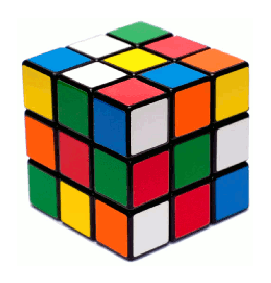
\includegraphics[width=2cm]{Geometrie_did/Images/Geo6_cours_Rubiks}}
   \psnode(6,17){F}{}
   %\ncline{F}{E}
   %Pyramide
   \psnode(14.75,14){C}{\begin{minipage}{4.5cm}{\bf Pyramide} : une base polygonale, un sommet, des faces latérales triangulaires, qui sont isocèles et superposables si la pyramide est régulière.\end{minipage}}
   \rput(15,17){\psSolid[object=tetrahedron,r=0.6,action=draw*,RotZ=70,linecolor=A1]}
   \rput(14.75,20.5){\includegraphics[width=4.5cm]{Geometrie_did/Images/Geo6_cours_Kheops}}
   \ncline{A}{C}
   \ncput*{\textcolor{A1}{pyramides}}
   %Cylindre
   \psnode(3.75,6.5){D}{\begin{minipage}{4.5cm}{\bf Cylindre} : du grec {\it kulindros}, rouleau. Deux bases en forme de disques, une surface latérale.\end{minipage}}
   \rput(4.5,3.5){\psSolid[object=cylindre,h=1,r=0.2,action=draw**,
ngrid=8 16,RotX=90,linecolor=B2]}
   \rput(3.75,1){\includegraphics[height=2.75cm]{Geometrie_did/Images/Geo6_cours_conserve}}
   \ncline{A}{D}
   \ncput*{\textcolor{B2}{cylindres}}
   %Cône
   \psnode(9.25,6.5){D}{\begin{minipage}{4.5cm}{\bf Cône} : du grec {\it kônos}, pomme de pain. Une base en forme de disque, une surface latérale, un sommet. \end{minipage}}
   \rput(9.25,4.85){\psSolid[object=cone,h=0.8,r=0.4,action=draw**,ngrid=8 16,RotX=200,linecolor=B2]
}
   \rput(10,1){\includegraphics[height=3cm]{Geometrie_did/Images/Geo6_cours_glace}}
   \ncline{A}{D}
   \ncput*{\textcolor{B2}{cônes}}
   %Sphère
   \psnode(14.75,6.5){D}{\begin{minipage}{4.5cm}{La \bf sphère} : du grec {\it sphaîra}, corps rond, est la surface extérieure de la {\bf boule}. \end{minipage}}
   \rput(14.75,4.15){\psSolid[object=sphere,r=0.45,ngrid=18 18,linecolor=B2]}
   \rput(14.75,1){\includegraphics[height=2.75cm]{Geometrie_did/Images/Geo6_cours_ballon}}
   \ncline{A}{D}
   \ncput*{\textcolor{B2}{boules}}
\end{pspicture}}




\subsection{Matériel pédagogique pour travailler avec les solides}

Il existe un matériel pédagogique bien adapté à la géométrie dans l'espace. On peut cependant tout à fait faire de la géométrie dans l'espace avec des objets usuels de la vie courante (boites de conserve, emballages, jouets\dots).

\smallskip

{\bf Kubix} : jeu de construction en bois pour développer l'imagination et travailler sur les solides. Assortiment de cubes, de prismes, de cylindres, de demi-cylindres, de pavés, de cônes tout en couleur.
\begin{center}
   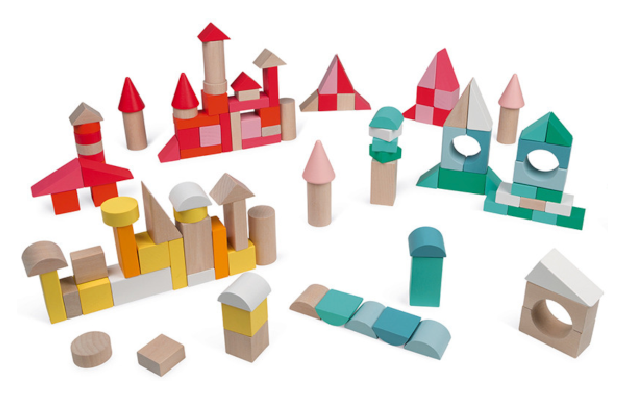
\includegraphics[width=7cm]{Geometrie_did/Images/Geo6_cours_kubics}
\end{center}

{\bf Solides prêts à l'emploi} : en bois ou en plastique, c'est un assortiment de différentes formes, qui permettent de décrire ces solides en les manipulant. Il en existe également en plastique transparent pouvant contenir un patron.
\begin{center}
   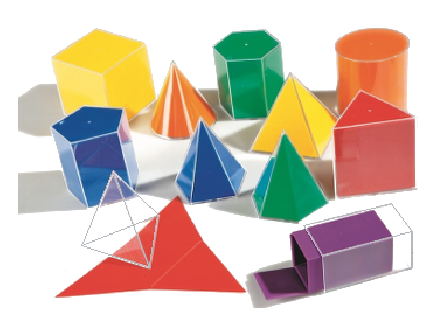
\includegraphics[width=4.5cm]{Geometrie_did/Images/Geo6_cours_solides}
\end{center}

{\bf Polydrons} : polygones en plastique, variés, qui peuvent être assemblés par leur arête pour construire des polyèdres. Il en existe également des sphériques afin de construire sphères, cylindres et cônes.
\begin{center}
   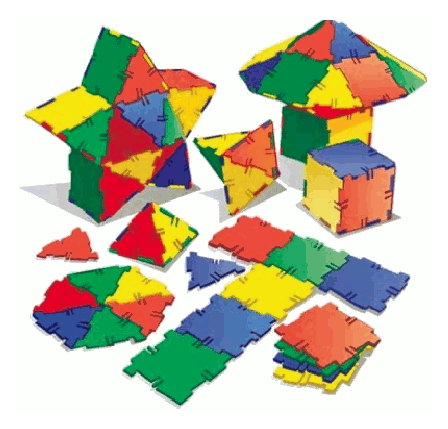
\includegraphics[width=4.5cm]{Geometrie_did/Images/Geo6_cours_polydrons}
\end{center}

{\bf Tiges et connecteurs} : en plastique, ou avec des pailles, des allumettes et de la pâte à modeler. Les tiges sont à imbriquer grâce à des connecteurs pour fabriquer des solides à partir de leurs arêtes.
\begin{center}
   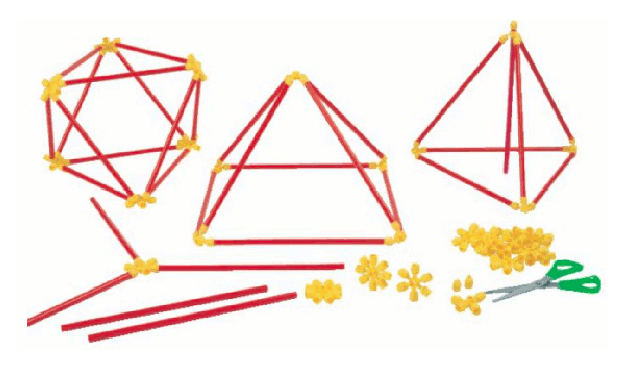
\includegraphics[width=5.5cm]{Geometrie_did/Images/Geo6_cours_tiges}
\end{center}

{\bf Cubes à emboiter} : petits cubes de plastique qui peuvent être assemblés par face, à l'aide de clips, pour construire des polyèdres et travailler sur les représentations de face, de côté et du dessus par exemple.
\begin{center}
   
\includegraphics[width=5cm]{Geometrie_did/Images/Geo6_cours_cubes}
\end{center}


\subsection{Quelques erreurs et difficultés des élèves} %%%

\smallskip

{\bf Au niveau de la reconnaissance et de la description}

Il s'agit pour l'élève de reconnaître des propriétés d'un solide : nombre de faces,  d'arêtes, de sommets, nature des faces, et en fonction de ces caractéristiques de lui donner un nom. Plusieurs cas peuvent se produire :
{\renewcommand{\StringDOCUMENTATION}{Difficultés}
\begin{documentation}
\begin{itemize}
   \item l'élève a le solide à sa disposition : il suffit de lire directement ses propriétés. Le risque est de compter deux fois des objets identiques ;
   \item l'élève voit le solide mais ne peut le manipuler ni tourner autour : il doit imaginer ce qu'il ne voit pas, ce qui suppose qu'il a déjà eu l'occasion de manipuler ce solide ;
   \item l'élève ne dispose que du tracé en perspective de ce solide : il faut qu'il connaisse et se soit approprié les conventions de la perspective cavalière. \\ [-7mm]
\end{itemize}
\end{documentation}}

\bigskip

{\bf Au niveau des patrons}

Deux types de tâches peuvent être proposées à l'élève : \\
   -- reconnaître si un dessin donné est le patron ou non d'un solide ; \\
   -- construire le patron du solide.

{\renewcommand{\StringDOCUMENTATION}{Difficultés}
\begin{documentation}
\begin{itemize}
   \item toutes les faces du solide doivent être représentées ;
   \item les côtés des différents polygones qui représentent les faces et qui se correspondent après pliage doivent être de même dimension ;
   \ item deux faces ne doivent pas se superposer ;
   \item si l'élève n'a  pas le droit de manipuler l'objet, il devra construire le patron en étalant mentalement les différentes faces de l'objet ;
   \item beaucoup d'élèves s'imaginent qu'un solide ne possède qu'un seul patron. \\ [-7mm]
\end{itemize}
\end{documentation}}


%%%%%%%%%%%%%%%%%%%%%%%%%%%%%
%%%%%%%%%%%%%%%%%%%%%%%%%%%%%
\activites

\textcolor{G1}{Sujet proposé aux M2 par la FDE de Montpellier, 2022} \\

{\bf\uline{Consigne}} : Vous êtes enseignant(e) en Grande Section de maternelle. Vous souhaitez mettre en œuvre une séquence permettant de faire acquérir la compétence \og Reconnaitre et nommer quelques formes planes (carré, triangle, cercle ou disque, rectangle) et ce dans toutes leurs orientations et configurations \fg. \\
   À partir de la ressource placée en annexe 1 et qui représente la première séance, présentez la deuxième séance de cette séquence, sous forme d’atelier dirigé, dont l’objectif est de passer d’une perception globale à une perception plus analytique du rectangle. \\

{\bf\uline{Compétence(s) et connaissance(s) visée(s)}} : Reconnaitre et nommer quelques formes planes (carré, triangle, cercle ou disque, rectangle) et ce dans toutes leurs orientations et configurations. \\

{\bf\uline{Contexte de la séance d'enseignement}} : \\
   \hspace*{5mm} -- cycle d'enseignement : cycle 1 ; \\
   \hspace*{5mm} -- niveau de la classe : GS ; \\
   \hspace*{5mm} -- domaine : Explorer des formes, des grandeurs, des suites organisées ; \\
   \hspace*{5mm} -- période : période 1. \\ [3mm]
  

{\bf\uline{Documents fournis au candidat}} : \\

{\bf\uline{Document 1}} : Extrait du programme consolidé de cycle 1 publié au BO n°25 du 24/06/2021. \medskip

\begin{center}
   \begin{minipage}{16cm}
      \textsf{{\bf 4.2. Explorer des formes, des grandeurs, des suites organisées} \\ [1mm]
      Très tôt, les jeunes enfants discernent intuitivement des formes (carré, triangle, etc.) et des grandeurs (longueur, contenance, masse, aire, etc.). À l’école maternelle, ils construisent des connaissances et des repères sur quelques formes et grandeurs. L’approche des formes planes, des objets de l’espace, des grandeurs, se fait par la perception visuelle, la manipulation et la coordination d’actions sur des objets. Cette approche est soutenue par le langage : il permet de décrire ces objets et ces actions et favorise l’identification de premières caractéristiques descriptives. Ces connaissances qui resteront limitées constituent une première approche de la géométrie et de la mesure qui seront enseignées aux cycles 2 et 3. \\ [2mm]
      {\bf 4.2.1. Objectifs visés et éléments de progressivité} \\ [1mm]
      Très tôt, les enfants regroupent les objets, soit en fonction de leur aspect, soit en fonction de leur utilisation familière ou de leurs effets. À l’école, ils sont incités à « mettre ensemble ce qui va ensemble » pour comprendre que tout objet peut appartenir à plusieurs catégories et que certains objets ne peuvent pas appartenir à celles-ci. \\
      Par des observations, des comparaisons, des tris, les enfants sont amenés à mieux distinguer différents types de critères : forme, longueur, masse, contenance essentiellement. Ils apprennent {\bf progressivement} à reconnaître, distinguer, décrire des solides puis des formes planes. Ils commencent à appréhender la notion d’alignement qu’ils peuvent aussi expérimenter dans les séances d’activités physiques. L’enseignant est attentif au fait que l’appréhension des formes planes est plus abstraite que celle des solides et que certains termes prêtent à confusion (carré/cube). L’enseignant utilise un vocabulaire précis (cube, boule, pyramide, cylindre, carré, rectangle, triangle, cercle ou disque - à préférer à « rond ») que les enfants sont entraînés ainsi à comprendre d’abord puis amenés progressivement à utiliser. \\
      Par ailleurs, {\bf dès la petite section}, les enfants sont invités à organiser des suites d’objets en fonction de critères de formes et de couleurs ; les premiers algorithmes qui leur sont proposés sont constitués d’alternances simples. {\bf Dans les années suivantes, progressivement}, ils sont amenés à reconnaître un rythme dans une suite organisée et à continuer cette suite, à inventer des \og rythmes \fg{} de plus en plus compliqués, à compléter des manques dans une suite organisée.}
   \end{minipage}
\end{center}

\begin{center}
   \begin{minipage}{16cm}
      \textsf{{\bf 4.2.2. Ce qui est attendu des enfants en fin d’école maternelle} \\ [1mm]
      -- Classer des objets en fonction de caractéristiques liées à leur forme. \\
      -- Reconnaître quelques solides (cube, pyramide, boule, cylindre). \\
      -- Savoir nommer quelques formes planes (carré, triangle, cercle ou disque, rectangle) et ce dans toutes leurs orientations et configurations. \\
      -- Classer ou ranger des objets selon un critère de longueur ou de masse ou de contenance. \\
      -- Reproduire un assemblage à partir d’un modèle (puzzle, pavage, assemblage de solides). \\
      -- Reproduire, dessiner des formes planes. \\
      -- Identifier une organisation régulière et poursuivre son application.}
   \end{minipage}
\end{center}

\bigskip


{\bf\uline{Document 2}} : Extrait de {\it Cap Maths GS}. Guide de l’enseignant, Hatier, 2015. pp. 54, 56 et 57. 

\begin{center}
   \fbox{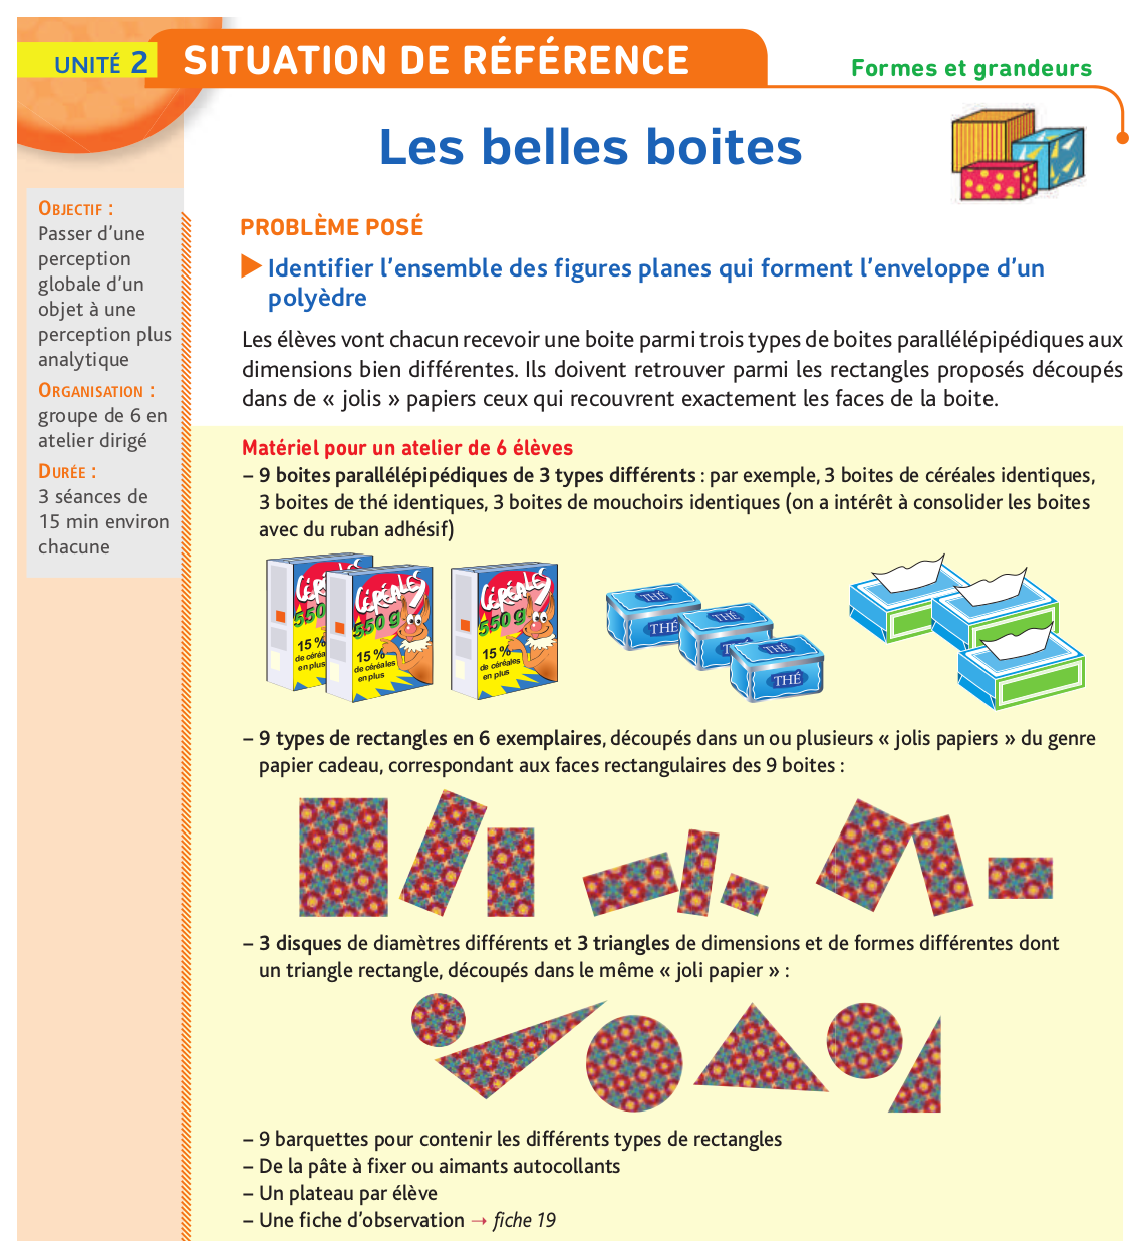
\includegraphics[width=15cm]{Geometrie_did/Images/Geo6_crpe_boites_1}} \\
   \fbox{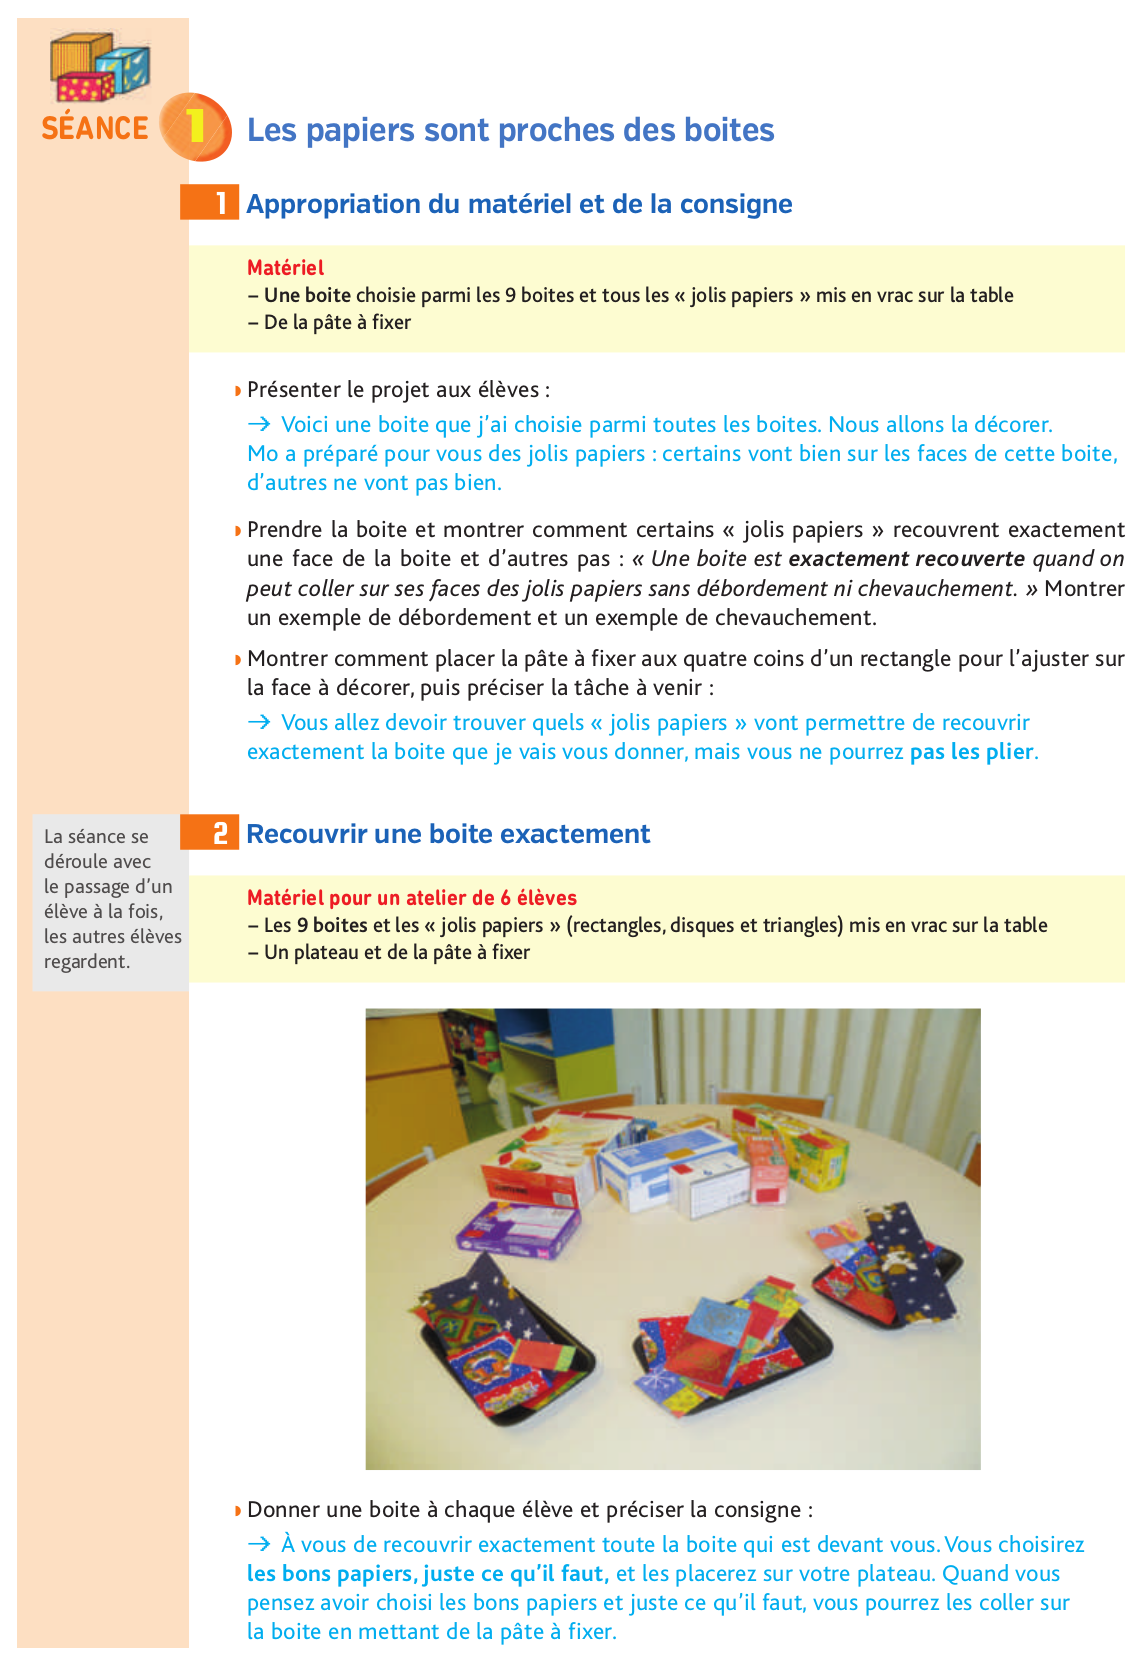
\includegraphics[width=15cm]{Geometrie_did/Images/Geo6_crpe_boites_2}} \\
   \fbox{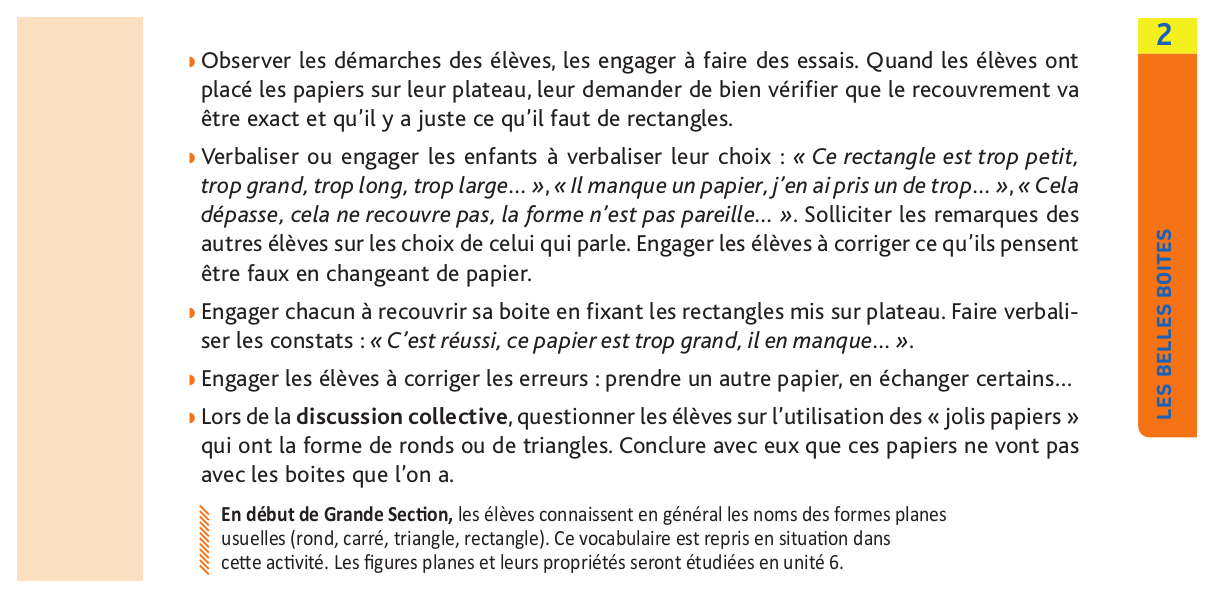
\includegraphics[width=15cm]{Geometrie_did/Images/Geo6_crpe_boites_3}}
\end{center}


%%%%%%%%%%%%%%%%%%%%%%%%%%
\analyses %%% 
%%%%%%%%

\begin{exercice}[Trions les emballages]
Des élèves de CE1 ont apporté en classe différents emballages présents dans le commerce :

A. différentes boites parallélépipédiques et cubiques ; \\
B. des prismes droits à bases triangulaires (Toblerone) ou octogonales ; \\
C. une pyramide à base carrée tronquée (boîte de fromage de chèvre) ; \\
D. des cylindres (boîtes de conserve diverses, boîte de camembert, rouleau de papier d'aluminium) ; \\
E. des cônes ; \\
F. des boules (balles, ballons) ; \\
G. d'autres emballages (formes ovales, anneaux, boîtes en forme de c\oe ur)

L'enseignant propose un déroulement de la séance suivant deux phases :
\begin{itemize}
   \item Phase 1 : chaque groupe d'élèves a reçu les mêmes types de solides. La tâche est de constituer des groupes de solides, de mettre ensemble ceux qui se ressemblent et d'écrire pourquoi on les a mis ensemble.
   \item Phase 2 : Mise en commun collective et discussion sur les classements effectués. Synthèse des résultats.
\end{itemize}

\begin{enumerate}
   \item Proposer un classement didactiquement pertinent (selon deux critères) des solides apportés en classe (différent des sept catégories déjà citées : A, B, C\dots). Classer alors les sept catégories suivant ces deux critères.
   \item Quels sont les solides présents dans les programmes du cycle 2? L'enseignant propose des solides non présents dans ce programme. Justifier son choix.
   \item En observant les élèves, l'enseignant leur précise très rapidement qu'il faut s'intéresser {\bf uniquement aux formes} des boites d'emballages. Pourquoi ?
   \item Lors de la phase 2, les catégories répertoriées sont : objets ronds, objets carrés, objets \og rectangles \fg, objets \og triangle \fg{} etc. Faire des hypothèses sur l'origine de ces types de réponses.
   \item Le rouleau de papier d'aluminium a provoqué des litiges au niveau des élèves. Pourquoi ?
   \item Analyser les productions des groupes 1 et 2 :
   
   \begin{center}
   \begin{tabular}{|C{5}|C{5}|}
      \hline
      Groupe 1 & Groupe 2 \\
      \hline
      \multicolumn{2}{|c|}{Ces groupes proposent de mettre ensemble :} \\
      \hline
      A, B et C & A, B et D \\
      F & C et E \\
      G & F et G \\
      \hline
   \end{tabular}
   \end{center}
   \item À la suite de cette première catégorisation, l'enseignant demande aux élèves de faire bouger les solides sur la table et de trier ceux qui roulent, et ceux qui ne roulent pas.
   \begin{enumerate}
      \item Émettre une hypothèse sur l'intention de l'enseignant.
      \item Ce critère est-il toujours pertinent ?
   \end{enumerate}
\end{enumerate}
\end{exercice}

\begin{corrige}
\ \\ [-5mm]
\begin{enumerate}
   \item On peut classer les solides suivant leur caractère polyédrique ou non :
   \begin{itemize}
      \item les polyèdres : A, B, C ;
      \item les non polyèdres : D, E, F, G. 
   \end{itemize}
   \item Dans les programme du cycle 2, les solides présents sont la boule, le cylindre, le cône, le cube, le pavé droit et la pyramide. Il s'agit de les reconnaître, les trier et les nommer. \\
   Cependant, il est important de présenter également d'autres types de solides afin de montrer qu'il en existe justement d'autres, et de pouvoir identifier les solides les uns par rapport aux autres ainsi que leurs caractéristiques principales. 
   \item Les élèves pourraient proposer un classement du type \og sucré, salé \fg{}, ou \og ça se mange - ça ne se mange pas \fg{} ou encore proposer un classement par couleur, par taille\dots. \\
   Si on ne précise pas qu'il faut s'intéresser uniquement aux formes des emballages, on peut donc obtenir une multitude de classements n'ayant aucun rapport avec ce que l'enseignant souhaite obtenir !
     \item Tout d'abord, le passage du plan à l'espace n'est pas forcément clair pour les élèves : ils sont beaucoup plus habitués à travailler dans le plan. \\
     Ensuite, ils ont eu l'habitude, notamment en maternelle, de reconnaître, classer et nommer des formes simples comme le carré, le triangle, le disque.
   \item Le rouleau de papier d'aluminium est un objet non fermé. Contrairement aux autres qui, même si on peut les ouvrir (comme les différentes boites), peuvent tous être complètement fermés.
   \item Pour le \textbf{groupe 1}, il semble que les élèves ont \og repéré \fg{} les polyèdres. Les boules forment une catégorie, les autres emballages une troisième catégorie. \\
   On remarque que les cylindres et les cônes n'apparaissent pas dans le classement, sûrement en raison de leur forme mélangeant des faces planes comme pour les polyèdres A, B, C et des surfaces non planes comme pour la sphère.  \\
   Pour le \textbf{groupe 2}, les élèves ont classé ensemble les prismes et les cylindres, c'est à dire les solides ayant des faces opposées parallèles ; puis les solides \og pointus \fg{} (pyramides et cônes) et enfin les boules et autres emballages, peut-être comme la catégorie des formes \og arrondies \fg{}, les cylindres et les cônes ayant déjà été classés. 
   \item 
   \begin{enumerate}
      \item Le but de l'enseignant est de les faire classer les objets selon si ce sont des polyèdres (ceux qui ne roulent pas) ou non (ceux qui roulent), et à cette occasion d'introduire le terme de polyèdre.
      \item Ce critère n'est cependant pas pertinent didactiquement : par exemple un cube ayant une face bombée vers l'intérieur ne roule pas. Pourtant, ce n'est pas un polyèdre. \\
      Inversement, un polyèdre régulier avec de multiples faces donne l'impression qu'il roule lorsqu'on le lance.
    \end{enumerate}
\end{enumerate}
\end{corrige}

\vfill
\pagebreak

\begin{exercice}[Programmation]
{\it D'après une activité testée dans une école de Saint-Denis 3, Réunion}. \\
Après avoir travaillé en littérature sur le douze travaux d'Hercule, et notamment le travail n\degre11 dans lequel Hercule doit dérober les pommes d'or du jardin d'Hespérides, on propose dans une classe de CM2 une activité de mathématiques s'y rapportant. \\
Les élèves sont regroupés par quatre et ont a leur disposition les huit cartes suivantes : \\

{\psset{unit=0.5}
\hspace*{-0.5cm}
\begin{pspicture}(0,-0.5)(8.5,9.5)
   \rput(4,9){\bf A}  
   \put(1,7){\dep} 
   \put(2,4){\td}
   \put(2,5){\av{2}}
   \put(1,3.5){\ret{3}}
   \put(1,2.5){\av{3}}
   \put(1,1.5){\fin}
\end{pspicture}
\begin{pspicture}(0,-0.5)(8.5,9.5)
   \rput(4,9){\bf B}
   \put(1,7){\dep}
   \put(1,6){\av{2}}
   \put(1,5){\tg}
   \put(1,4){\tg}
   \put(1,3){\tg}
   \put(1,2){\tg}
   \put(1,1){\av{2}}
   \put(1,0){\fin}
\end{pspicture}
\begin{pspicture}(0,-0.5)(8.5,9.5)
   \rput(4,9){\bf C}
   \put(1,7){\dep}
   \put(1,6){\av{1}}
   \put(1,5){\tg}
   \put(1,4){\av{2}}
   \put(1,3){\td}
   \put(1,2){\av{2}}
   \put(1,1){\av{1}}
   \put(1,0){\fin}
\end{pspicture}
\begin{pspicture}(0,-0.5)(8.5,9.5)
   \rput(4,9){\bf D}
   \put(1,7){\dep}  
   \put(2,5){\td}
   \put(1,4.5){\reo{4}}
   \put(2,2.5){\av{2}}
   \put(2,1.5){\tg}
   \put(1,1){\ret{2}}
   \put(1,0){\av{4}}
   \put(1,-1){\fin}
\end{pspicture}

\hspace*{-0.75cm}
\begin{pspicture}(-0.5,-1)(8.5,10.5)
   \rput(4,9){\bf 1}
   \psgrid[subgriddiv=1,gridlabels=0](0,0)(8,8)
    \put(2.1,2.1){\ho} \put(0.1,4.1){\po}
    \put(5,3){\cn} \put(7,7){\cn} \put(3,6){\cn} \put(0,6){\cn}  \put(5,5){\cn} \put(2,1){\cn} \put(2,5){\cn} \put(6,2){\cn} \put(1,3){\cn}     
\end{pspicture}
\begin{pspicture}(-0.5,-1)(8.5,10.5)
   \rput(4,9){\bf 2}
   \psgrid[subgriddiv=1,gridlabels=0](0,0)(8,8)
    \put(6.1,2.1){\reflectbox{\ho}} \put(6.1,1.1){\po}
    \put(7,6){\cn} \put(3,3){\cn} \put(3,6){\cn} \put(2,5){\cn} \put(5,3){\cn} \put(5,5){\cn} \put(1,3){\cn} \put(0,0){\cn} \put(2,5){\cn}    
\end{pspicture} 
\begin{pspicture}(-0.5,-1)(8.5,10.5)
   \rput(4,9){\bf 3}
     \psgrid[subgriddiv=1,gridlabels=0](0,0)(8,8)
    \put(3.1,4.1){\ho} \put(7.1,6.1){\po}
    \put(1,1){\cn} \put(2,3){\cn} \put(3,2){\cn} \put(2,4){\cn}  \put(5,5){\cn} \put(7,2){\cn} \put(5,7){\cn} \put(6,0){\cn} \put(1,6){\cn}  
\end{pspicture}
\begin{pspicture}(-0.5,-1)(8.5,10.5)
   \rput(4,9){\bf 4}
   \psgrid[subgriddiv=1,gridlabels=0](0,0)(8,8)
    \rput{90}(2.5,3.5){\ho} \put(2.1,7.1){\po}
    \put(5,3){\cn} \put(3,3){\cn} \put(3,6){\cn} \put(0,5){\cn}  \put(7,5){\cn} \put(2,1){\cn} \put(2,0){\cn} \put(6,2){\cn} \put(1,3){\cn}
\end{pspicture}}
Les quatre cartes A, B, C et D proposent un programme de déplacement, les quatre cartes 1, 2, 3 et 4 sont constituées d'un quadrillage dans lequel trois sortes de cases sont représentées :
\begin{itemize}
   \item des cases noires, par lesquelles on ne peut pas passer (ce sont des murs) ;
   \item une case avec un personnage : il s'agit d'Hercule ;
   \item une case avec le pommier aux pommes d'or.
\end{itemize}
Les élèves doivent associer un programme à son quadrillage : l'association est réussie si, lorsqu'on déroule l'algorithme du programme, le personnage d'Hercule arrive effectivement au pommier.
\begin{enumerate}
   \item Dans quel domaine mathématique se situe-t-on ?
   \item Résoudre l'activité proposée aux élèves en expliquant la procédure utilisée.
   \item Citer deux compétences requises pour faire cette activité en CM2 ?
   \item Citer deux difficultés prévisibles.
   \item Quelle aide matérielle peut-on proposer à des élèves qui n'arriveraient pas à résoudre l'activité ?
   \item Dans un second temps, on propose aux groupes d'élèves de créer, pour chaque programme, un programme équivalent comportant un minimum d'instructions (sans nécessairement passer par le même chemin, mais ayant même départ et même arrivée). Quelles seraient ces programmes ?
\end{enumerate}
\end{exercice}

\begin{corrige}
\ \\ [-5mm]
\begin{enumerate}
   \item Le thème étudié ici est le codage et la programmation, et plus particulièrement \og coder le déplacement d'un personnage sur un quadrillage \fg{}, dans le domaine \og espace et géométrie \fg.
   \item On peut par exemple choisir l'une des cartes \og programme \fg{}. Pour cette carte, on teste le programme sur le quadrillage 1, puis 2\dots {} jusqu'à trouver la bonne association. On poursuit de la même façon avec les autres cartes programme. On obtient : A - 2 \quad ; \quad B - 4 \quad ; \quad C - 3 \quad D - 1.
   \item Compétences requises :
   \begin{itemize}
      \item se repérer, décrire ou exécuter des déplacements, sur un
plan ou sur une carte ;
      \item connaître et utiliser le vocabulaire permettant de définir des
positions et des déplacements.
   \end{itemize}
   \item Exemples de difficultés :
   \begin{itemize}
      \item mauvaise compréhension de la consigne ;
      \item difficultés d'orientations (repérage relatif, dans un plan) ;
      \item choix de la procédure à utiliser pour arriver à ses fins.
   \end{itemize}
   \item On peut proposer à des élèves un quadrillage plus grand sur une feuille A4 avec un personnage de type Playmobil (donc orienté et pouvant se tenir debout) représentant Hercule ainsi qu'un jeton pour le pommier. L'élève devra tout d'abord placer le personnage et le jeton, puis tester les déplacements. L'avantage de ce matériel est un retour à une représentation en 3D, plus proche de la réalité et donc plus facilement transposable à la réalité. \\
   \hspace*{3cm} 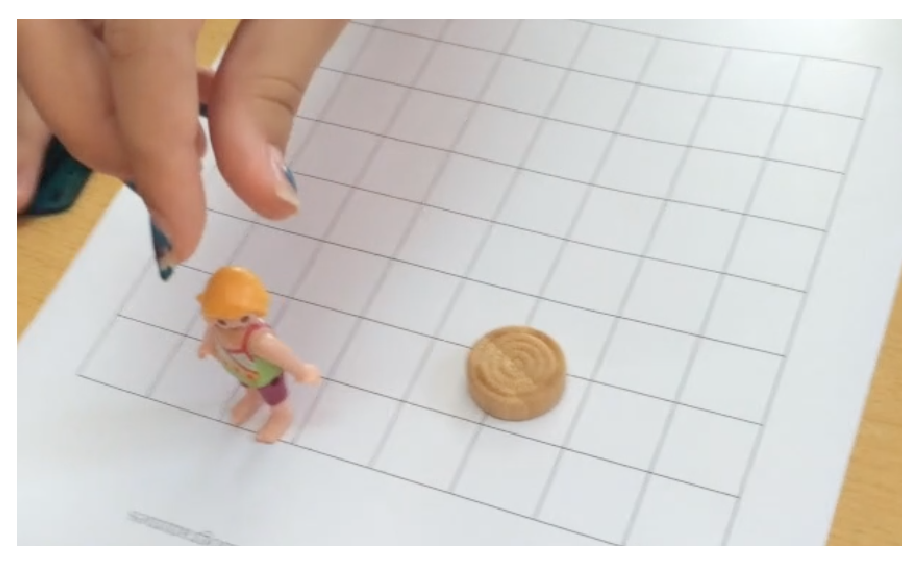
\includegraphics[width=11cm]{Geometrie_did/Images/Geo6_analyse_Playmobil} \\
   On peut également faire le même type d'action sur une nappe quadrillée sur laquelle les élèves peuvent se déplacer.
   \item On obtient les programmes minimum suivants : \\
   {\psset{unit=0.5}
   \hspace*{-0.5cm}
   \begin{pspicture}(0,2)(8,9.5)
      \rput(4,8.5){\bf A}  
      \put(1,7){\dep} 
      \put(1,6){\tg}
      \put(1,5){\av{1}}
      \put(1,4){\fin}
   \end{pspicture}
   \begin{pspicture}(0,2)(8,9.5)
      \rput(4,8.5){\bf B}
      \put(1,7){\dep}
      \put(1,6){\av{4}}
      \put(1,5){\fin}
   \end{pspicture}
   \begin{pspicture}(0,2)(8,9.5)
      \rput(4,8.5){\bf C}
      \put(1,7){\dep}
      \put(1,6){\av{4}}
      \put(1,5){\tg}
      \put(1,4){\av{2}}
      \put(1,3){\fin}
   \end{pspicture}
   \begin{pspicture}(0,2)(7,9.5)
      \rput(4,8.5){\bf D}
      \put(1,7){\dep}  
      \put(1,3.5){\ret{2}}
      \put(2,5){\tg}
      \put(2,4){\av{2}}
      \put(1,2.5){\fin}
   \end{pspicture}}
\end{enumerate}
\end{corrige}

\vfill
\pagebreak

\begin{exercice}[CRPE 2005 Créteil] %%%%%
\begin{enumerate}
   \item Quelles sont les intentions d'un enseignant qui utiliserait l'ensemble des documents suivants :
   \begin{itemize}
      \item Document 1 : Extrait de Diagonale, livre du maître 2002, CE2.
      \item Document 2 : Exercice 1 (extrait de Diagonale, livre de l'élève 2002, CE2), et exercices 2, 3 et 4 (extraits de Euro-Maths CE2, 2003).
   \end{itemize}
   \item Dans le document extrait du livre du maître (Document 1), il est demandé de donner une signification du mot « patron ». Que donneriez-vous comme signification aux élèves ?
   \item Expliquer sans avoir à découper réellement pourquoi les assemblages b, c, d (exercice 1, document 2) ne sont pas des patrons de cubes (on aura intérêt à mettre en place un codage pour expliquer).
   \item Comparer les exercices 1 et 2 (document 2) aux niveaux : de la présentation, de la consigne, de la vérification.
   \item Comment justifier l'exercice 3 après avoir travaillé sur l'exercice 2 ?
   \item Comment justifier l'exercice 4 après avoir proposé de travailler sur l'exercice 2 ?
\end{enumerate}

\fbox{
\begin{minipage}{16.5cm}
\begin{center}
   {\Large\bf Document 1}
\end{center}
\begin{minipage}{11.5cm}
MATERIEL :
\begin{itemize}
    \item le livre de l'élève page 131 ;
    \item une vingtaine de carrés (de quatre carreaux sur quatre) par groupe de deux élèves ;
   \item des morceaux d'adhésif repositionnables ;
   \item une paire de ciseaux ;
   \item une feuille de papier quadrillé. \\
\end{itemize}
\end{minipage}
\qquad
\begin{minipage}{4cm}
   {\small
   Remarques : \\
   $\bullet$ Utiliser des feuilles rigides (fiches de bristol) pour faciliter les manipulations. On peut faire découper les carrés par les élèves.}
\end{minipage}
{\bf 1\up{ère} phase : fabriquer des assemblages de carrés.} \\
\begin{minipage}{11.5cm}
$\bullet$ Regrouper les élèves par deux et leur demander d'assembler des carrés  pour obtenir un patron d'un cube. Leur préciser les étapes du travail : \\
   -- recherche et réalisation d'un assemblage ; \\
   -- reproduction de l'assemblage sur la feuille quadrillée (un carreau représentant une face) ; \\
   -- validation par construction d'un cube ; \\
   -- en cas de réussite, inscription de OUI à côté de la reproduction de l'assemblage fait sur la feuille, dans le cas contraire, inscription de NON. Faire rechercher ainsi divers assemblages et vérifier s'il s'agit de patrons d'un cube ou non. \\
$\bullet$ Partager le tableau en deux parties : une colonne pour les bons patrons, une autre pour les mauvais patrons. Collectivement, demander aux élèves de venir, équipe après équipe, faire une nouvelle proposition d'assemblage et de la  dessiner dans la bonne colonne (bon ou mauvais patron). \\
$\bullet$ Quand cinq ou six assemblages figurent au tableau, inviter les élèves à les observer et à formuler des remarques, en particulier par rapport aux raisons qui font que les assemblages de la colonne mauvais patrons ne conviennent pas.
\end{minipage}
\qquad
\begin{minipage}{4cm}
{\small
   $\bullet$ Rappeler la signification du mot \og patron \fg. \\
   $\bullet$ Pour fixer les faces entre elles, inviter les élèves à utiliser de petites bandes d'adhésif repositionnable. \\
   $\bullet$ Dans ce travail, les élèves seront amenés à faire certains constats dans la construction du cube. \\
   $\bullet$ Il ne s'agit pas d'obtenir de façon exhaustive tous les patrons d'un cube, mais de permettre aux élèves de relever des informations permettant d'éliminer certains assemblages, de reconnaitre les caractéristiques de bons patrons. \\}
\end{minipage}
\end{minipage}
}

\vfill
\pagebreak

\fbox{
\begin{minipage}{16.5cm}
\begin{center}
   {\Large\bf Document 2}
\end{center}
{\bf Exercice 1} \\
Trouve les deux assemblages de carrés qui permettent de construire un cube. Reproduis-les.
\begin{center}
{\psset{unit=0.8}
\begin{pspicture}(0,0)(16,7.5)
   \rput(3,6){\psSolid[object=parallelepiped,a=0.5,action=draw*,RotZ=-8,RotX=3]} 
   \face{1}{1} \face{2}{1} \face{3}{1} \face{4}{1} \face{5}{1} \face{2}{2} \face{4}{0}
   \face{7}{1} \face{8}{1} \face{9}{1} \face{8}{2} \face{9}{2} \face{9}{0}
   \face{11}{1} \face{12}{1} \face{13}{1} \face{14}{1} \face{14}{2} \face{14}{0}
   \face{6}{5} \face{7}{5} \face{8}{5} \face{7}{6} \face{8}{5} \face{9}{4} \face{8}{4}
   \face{11}{5} \face{12}{5} \face{13}{5} \face{14}{5} \face{14}{6} \face{12}{6}
   \rput(7.5,7.5){\bf a}
   \rput(13.5,7.5){\bf b}
   \rput(2.5,3.5){\bf c}
   \rput(9,3.5){\bf d}
   \rput(13.5,3.5){\bf e}
\end{pspicture}}
\end{center}

{\bf Exercice 2} \\
Quelles figures te permettent de reconstituer un cube ? Vérifie en essayant de construire le cube, après avoir reproduit les figures. Utilise du papier quadrillé.
\begin{center}
{\psset{unit=0.5}
\begin{pspicture}(0,0)(28,5) 
   \pspolygon(0,0)(1,0)(1,1)(3,1)(3,0)(4,0)(4,2)(0,2)
   \psline[linestyle=dashed](0,1)(1,1)(1,2)
   \psline[linestyle=dashed](2,1)(2,2)
   \psline[linestyle=dashed](3,2)(3,1)(4,1)
   \rput(0.5,2.5){A}
   \pspolygon(4,3)(6,3)(6,2)(7,2)(7,3)(8,3)(8,4)(7,4)(7,5)(6,5)(6,4)(4,4)(4,3)
   \psframe[linestyle=dashed](6,3)(7,4)
   \psline[linestyle=dashed](5,3)(5,4)
   \rput(4.5,4.5){B}
   \pspolygon(8,0)(11,0)(11,1)(13,1)(13,2)(10,2)(10,1)(8,1)
   \psline[linestyle=dashed](10,0)(10,1)(11,1)(11,2)
   \psline[linestyle=dashed](9,0)(9,1)
   \psline[linestyle=dashed](12,1)(12,2)
   \rput(8.5,1.5){C}
   \pspolygon(13,4)(14,4)(14,3)(15,3)(15,2)(17,2)(17,3)(16,3)(16,4)(15,4)(15,5)(13,5)
   \psline[linestyle=dashed](14,5)(14,4)(15,4)(15,3)(16,3)(16,2)
   \rput(12.5,4.5){D}
   \pspolygon(18,5)(21,5)(21,4)(20,4)(20,1)(19,1)(19,4)(18,4)
   \psline[linestyle=dashed](19,5)(19,4)(20,4)(20,5)
   \psline[linestyle=dashed](19,3)(20,3)
   \psline[linestyle=dashed](19,2)(20,2)
   \rput(17.5,4.5){E}
   \pspolygon(22,4)(22,1)(23,1)(23,2)(24,2)(24,5)(23,5)(23,4)
   \psline[linestyle=dashed](22,2)(23,2)(23,3)(22,3)
   \psline[linestyle=dashed](24,3)(23,3)(23,4)(24,4)
   \rput(22.5,4.5){F}
   \pspolygon(25,0)(26,0)(26,1)(29,1)(29,3)(28,3)(28,2)(25,2)   
   \psline[linestyle=dashed](25,1)(26,1)(26,2)
   \psline[linestyle=dashed](27,1)(27,2)
   \psline[linestyle=dashed](28,1)(28,2)(29,2)
   \rput(25.5,2.5){G}
\end{pspicture}}
\end{center}

{\bf Exercice 3} \\
À quel cube correspond ce patron ? Vérifie en construisant le cube après avoir reproduit le patron sur du papier quadrillé. 
\begin{center}
{\psset{unit=0.8}
\begin{pspicture}(-0.5,0.5)(11,4.5)
   \rput(4.2,3.8){$a$}
   \rput(6.2,1.5){$b$}
   \rput(8.7,3.5){$c$}
   \rotatebox{20}{
      \psframe[fillstyle=crosshatch](0,1)(1,2)
      \psframe[fillstyle=hlines,hatchangle=90](1,1)(2,2)
      \psframe[fillstyle=solid,fillcolor=lightgray](2,1)(3,2)
      \psframe(3,1)(4,2)
      \psframe[fillstyle=solid,fillcolor=black](2,2)(3,3)
      \psframe(2,0)(3,1)}  
   \rput(5,3){\rotatebox{20}{
      \psframe(0,0)(1,1)
      \pspolygon[fillstyle=hlines,hatchangle=90,hatchsep=0.09](1,0)(1.4,0.4)(1.4,1.4)(1,1)
      \pspolygon[fillstyle=crosshatch](0,1)(1,1)(1.4,1.4)(0.4,1.4)}}
   \rput(7,1){\rotatebox{-10}{
      \psframe[fillstyle=crosshatch](0,0)(1,1)
      \pspolygon[fillstyle=solid,fillcolor=black](0,0)(0,1)(-0.4,1.4)(-0.4,0.4)
      \pspolygon(0,1)(1,1)(0.4,1.4)(-0.4,1.4)}}
   \rput(9,4){\rotatebox{-70}{
      \psframe[fillstyle=solid,fillcolor=gray](0,0)(1,1)
      \pspolygon[fillstyle=hlines,hatchangle=90,hatchsep=0.09](1,0)(1.4,0.4)(1.4,1.4)(1,1)
      \pspolygon(0,1)(1,1)(1.4,1.4)(0.4,1.4)}}
\end{pspicture}}
\end{center}

{\bf Exercice 4} \\
\begin{minipage}{7cm}
{\psset{unit=0.8}
\begin{pspicture}(-2,-0.5)(6,3.3)
   \face{1}{0} \face{1}{1} \face{1}{2} \face{2}{1} \face{3}{1} \face{4}{1}
\end{pspicture}}
\end{minipage}
\begin{minipage}{7cm}
   Sur un dé à jouer, la somme des points inscrits sur deux faces opposées est 7. Inscrits les points sur le patron. Puis, vérifie tes prévisions en construisant le dé.
\end{minipage}
\end{minipage}}
\end{exercice}

\begin{corrige}
\ \\ [-5mm]
\begin{enumerate}
   \item Les intentions du maître sont de :
   \begin{itemize}
      \item faire émerger les caractéristiques d'un patron de cube ;
      \item faire reconnaître un patron de cube parmi différentes représentations ;
      \item faire travailler le passage du plan (le patron) à l'espace. 
   \end{itemize}
   \item Un \og patron \fg{} d'un solide est une surface plane d'un seul tenant qui, par pliage, permet de reconstituer le solide, sans recouvrement de ses faces. 
   \item
   \begin{itemize}
      \item L'assemblage {\bf c} n'est pas un patron du cube parce qu'il comporte sept carrés au lieu de six.
      \item Pour l'assemblages {\bf b}, les deux carrés \og du dessus \fg{} vont se chevaucher lorsqu'on va reconstituer le solide.
      \item Pour l'assemblage {\bf d}, les quatre carrés en haut à droite forment un carré ce qui est impossible puisque la somme des angles issus du sommet commun vaut $4\times90^\circ = 360^\circ$, les quatre faces sont dans le même plan.
   \end{itemize}   
   \item {\bf Concernant la présentation :} 
   \begin{itemize}
      \item dans l'exercice 1, on a en plus la présence d'un cube représenté en perspective ;
      \item l'exercice 1 comporte cinq assemblages alors qu'il y en a sept dans l'exercice 2 ;
      \item dans l'exercice 2, les \og traits de pliage \fg{} sont représentés par des pointillés alors que ce sont des traits pleins dans l'exercice 1 ;
      \item les figures sont plus grandes dans l'exercice 1 que dans l'exercice 2 ;
      \item dans l'exercice 1, l'un des assemblages est formé de sept carrés alors que tous ceux de l'exercice 2 n'en possèdent que six.
   \end{itemize}
   {\bf Concernant la consigne :}
   \begin{itemize}
      \item le statut des objets : dans l'exercice 1, on parle d'assemblages de carrés, alors que dans l'exercice 2 on parle de figures ;
      \item la formulation : dans l'exercice 1, la question est fermée, il s'agit de trouver les deux seuls patrons de cube. Dans l'exercice 2, le nombre de solutions n'est pas indiqué ;
      \item la réponse attendue : dans l'exercice 1, les élèves doivent reproduire deux assemblages, alors que dans l'exercice 2, ils doivent reproduire sur papier quadrillé les figures permettant de construire le cube et vérifier en essayant de le construire effectivement.
   \end{itemize}
   {\bf Concernant la vérification :}
   \begin{itemize}
      \item dans l'exercice 1 aucune vérification n'est évoquée ;
      \item à contrario, dans l'exercice 2, l'élève doit vérifier ses propositions par reconstruction du cube à partir des patrons. La reproduction de ces patrons est facilitée par l'utilisation du papier quadrillé.
   \end{itemize}
   \item Dans l'exercice 2, il est demandé à l'élève d'anticiper le résultat d'une construction à partir du patron du solide en repérant les éventuelles superpositions de faces. Dans l'exercice 3, il s'agit de situer des faces voisines du cube les unes par rapport aux autres sur le patron et dans une représentation en perspective. La résolution de l'exercice 3 nécessite le passage d'une représentation du cube en dimension 2 à une représentation du cube en dimension 3. Cet exercice peut donc être considéré comme un prolongement de l'exercice 2, à condition que les élèves aient au préalable travaillé la lecture de représentations en perspective.
   \item À l'issue de l'exercice 2, l'élève possède un patron de cube à partir de la figure E, patron qu'il peut manipuler pour reconstruire le dé. Dans l'exercice 4, il s'agit de repérer les faces opposées et la vérification se fait par construction. Ainsi, proposer l'exercice 4 à la suite de l'exercice 2, permet une continuité de l'apprentissage : reconnaître des patrons du cube, puis travailler plus précisément sur les positions relatives des différentes faces d'un de ces patrons.
\end{enumerate}
\end{corrige}

\pagebreak

\begin{exercice}[CRPE 2010 G2]
Dans une séquence sur les patrons de solides avec ses élèves de CM1, un enseignant met en \oe uvre deux activités proposées dans l’ouvrage \og Apprentissages géométriques et résolution de problèmes \fg{} (ERMEL, Hatier 2006).

\begin{minipage}{11cm}
{\bf Première activité.} \\
\underline{Description rapide de la séance :} \og {\it Les élèves doivent construire, dans un premier temps, des schémas correspondant au patron d’un solide non usuel : le cube tronqué (ci-contre). Les schémas font l’objet d’une mise en commun, les élèves doivent ensuite construire ce patron à l’aide de gabarits.} \fg
\end{minipage}
\begin{minipage}{6cm}
{\psset{unit=0.8}
\begin{pspicture}(-1.5,-1)(4.5,5.5)
   \pspolygon(0,0)(3,0)(4.5,1.5)(4.5,4.5)(1.5,4.5)(0.75,3.75)(0,1.5)
   \psline(3,0)(3,3)(4.5,4.5)
   \psline(0,1.5)(1.5,3)(0.75,3.75)
   \psline(1.5,3)(3,3)
   \rput(2.25,3){X}
   \rput(0,0.75){X}
   \rput(1.125,4.125){\rotatebox{45}{X}}
\end{pspicture}}
\end{minipage}

\underline{Objectifs de la séance :} \og {\it Amener les élèves à anticiper pour reconnaître si un assemblage de figures planes constitue ou non un patron. Ils doivent également reconnaître si deux patrons différents correspondent ou non à un même solide.} \fg

En début de séance, l’enseignant montre aux élèves le cube tronqué qu’il laissera visible par tous jusqu’à la fin du travail. La séance se déroule en deux phases.

\underline{Première phase :} les élèves doivent dessiner à main levée des schémas correspondant à des patrons du cube tronqué présenté. Cette phase est suivie d’une mise en commun qui permet de mettre en évidence des caractéristiques que tout patron valide doit posséder.
\begin{enumerate}
   \item Citer trois caractéristiques parmi celles qui pourront ainsi être dégagées.
\end{enumerate}

\medskip

\underline{Deuxième phase :} les élèves doivent construire effectivement un patron du cube tronqué.
\begin{enumerate}
\setcounter{enumi}{1}
   \item
   \begin{enumerate}
      \item  Lors de cette phase, l’enseignant fournit aux élèves des gabarits de différentes formes planes dont celles des faces du cube tronqué (chaque gabarit est en un seul exemplaire par élève). Donner deux arguments pouvant justifier ce choix.
      \item Certains élèves peuvent rencontrer des difficultés à réaliser le patron de ce solide. Citer deux aides matérielles que l’enseignant peut leur fournir.
   \end{enumerate}
\end{enumerate}

\medskip

{\bf Deuxième activité.} \\
L’enseignant demande à ses élèves d’assembler par quatre les cubes tronqués construits précédemment (voir ci-dessous) et de réaliser le patron du solide qui permettra de \og boucher le trou \fg.
\begin{center}
   \begin{pspicture}(0,0)(7,4)
      \pspolygon(0,0)(4,0)(7,1.5)(7,3.5)(3,3.5)(0,2)
      \psline(0,2)(4,2)(7,3.5)
      \psline(2,0)(2,2)(3,2.5)(4.5,2.75)(5.5,2.75)(5.5,0.75)
      \psline(1.5,2.75)(2.5,2.75)(4,3)(5,3.5)
      \psline(3,2.5)(2.5,2.75)
      \psline(4,3)(4.5,2.75)
      \psline[linestyle=dashed](0,0)(3,1.5)(7,1.5)
      \psline[linestyle=dashed](3,3.5)(3,1.5)
      \psline[linestyle=dashed](1.5,2.75)(1.5,0.75)(5.5,0.75)
      \psline[linestyle=dashed](2,0)(5,1.5)(5,3.5)
      \psline[linestyle=dashed](3.5,0.75)(3.5,1.75)
      \psline[linestyle=dashed](3,2.5)(3.5,1.75)(2.5,2.75)
      \psline[linestyle=dashed](4.5,2.75)(3.5,1.75)(4,3)
   \end{pspicture}
\end{center}
\begin{enumerate}
\setcounter{enumi}{2}
   \item Quelle est la difficulté particulière de cette activité pour les élèves ?
   \item À l’issue de ces deux activités, l’enseignant fait une synthèse sur la notion de patron. Donner une formulation de la trace écrite qui pourrait être proposée aux élèves.
\end{enumerate}
\end{exercice}

\begin{corrige}
\ \\ [-5mm]
\begin{enumerate}
   \item \textcolor{A2}{$\bullet$} Le patron doit avoir autant de faces que l’objet réel ;
   \begin{itemize}
      \item les formes des faces du patron doivent être les mêmes que celles de l’objet réel ;
      \item le patron doit être d'un seul tenant ;
      \item les faces ne doivent pas se recouvrir. \\
   \end{itemize}
   \item
   \begin{enumerate}
      \item \textcolor{A2}{$\bullet$} des gabarits de faces sont donnés, mais en nombre supplémentaire. Cela oblige l'élève à analyser le solide afin de ne choisir que les faces convenables ;
      \begin{itemize}
         \item les gabarits des faces du cube tronqué sont donnés. Cela libère les élèves de la complexité du tracé de certaines faces. Une fois ces gabarits trouvés, l'élève pourra mieux se concentrer sur l’analyse du solide, le nombre et la nature de ses faces et la disposition à adopter pour obtenir un patron ;
         \item chaque gabarit est en un seul exemplaire. Si le maître fournissait les sept gabarits correspondant aux sept faces, la tâche des élèves serait réduite à les disposer correctement. \\
      \end{itemize}
      \item \textcolor{A2}{$\bullet$} si la difficulté porte sur le choix des faces, le maître peut proposer aux élèves de manipuler le cube tronqué, de le comparer aux gabarits qu'il possède ;
      \begin{itemize}
         \item si la difficulté porte sur l'assemblage des gabarits, il peut proposer de donner plusieurs gabarits de même forme afin qu'il puisse avoir autant de faces que de gabarits ;
         \item il peut aussi proposer d'encrer les faces du cube tronqué afin de créer un patron sur une feuille et de s'inspirer de ce patron pour tracer le sien. \\
      \end{itemize}
   \end{enumerate}
   \item La difficulté particulière de cette activité vient du fait que le solide à construire n’est pas un objet matériel, on doit imaginer qu’il bouche le trou. Cela entraîne entre autre l’impossibilité de le tourner dans tous les sens pour l’observer (et par exemple de placer la pyramide dans sa position la plus usuelle, sommet en haut). \\
   \item On pourrait proposer la trace écrite suivante : \og Le patron d’un solide est une surface plane d’un seul tenant qui, par pliage, permet de reconstituer le solide sans recouvrement de ses faces. \fg{}
\end{enumerate}
\end{corrige}

\bigskip

\begin{exercice}[CRPE 2017 G3]
Un enseignant propose l’exercice ci-dessous à des élèves de CM1.

\begin{center}
   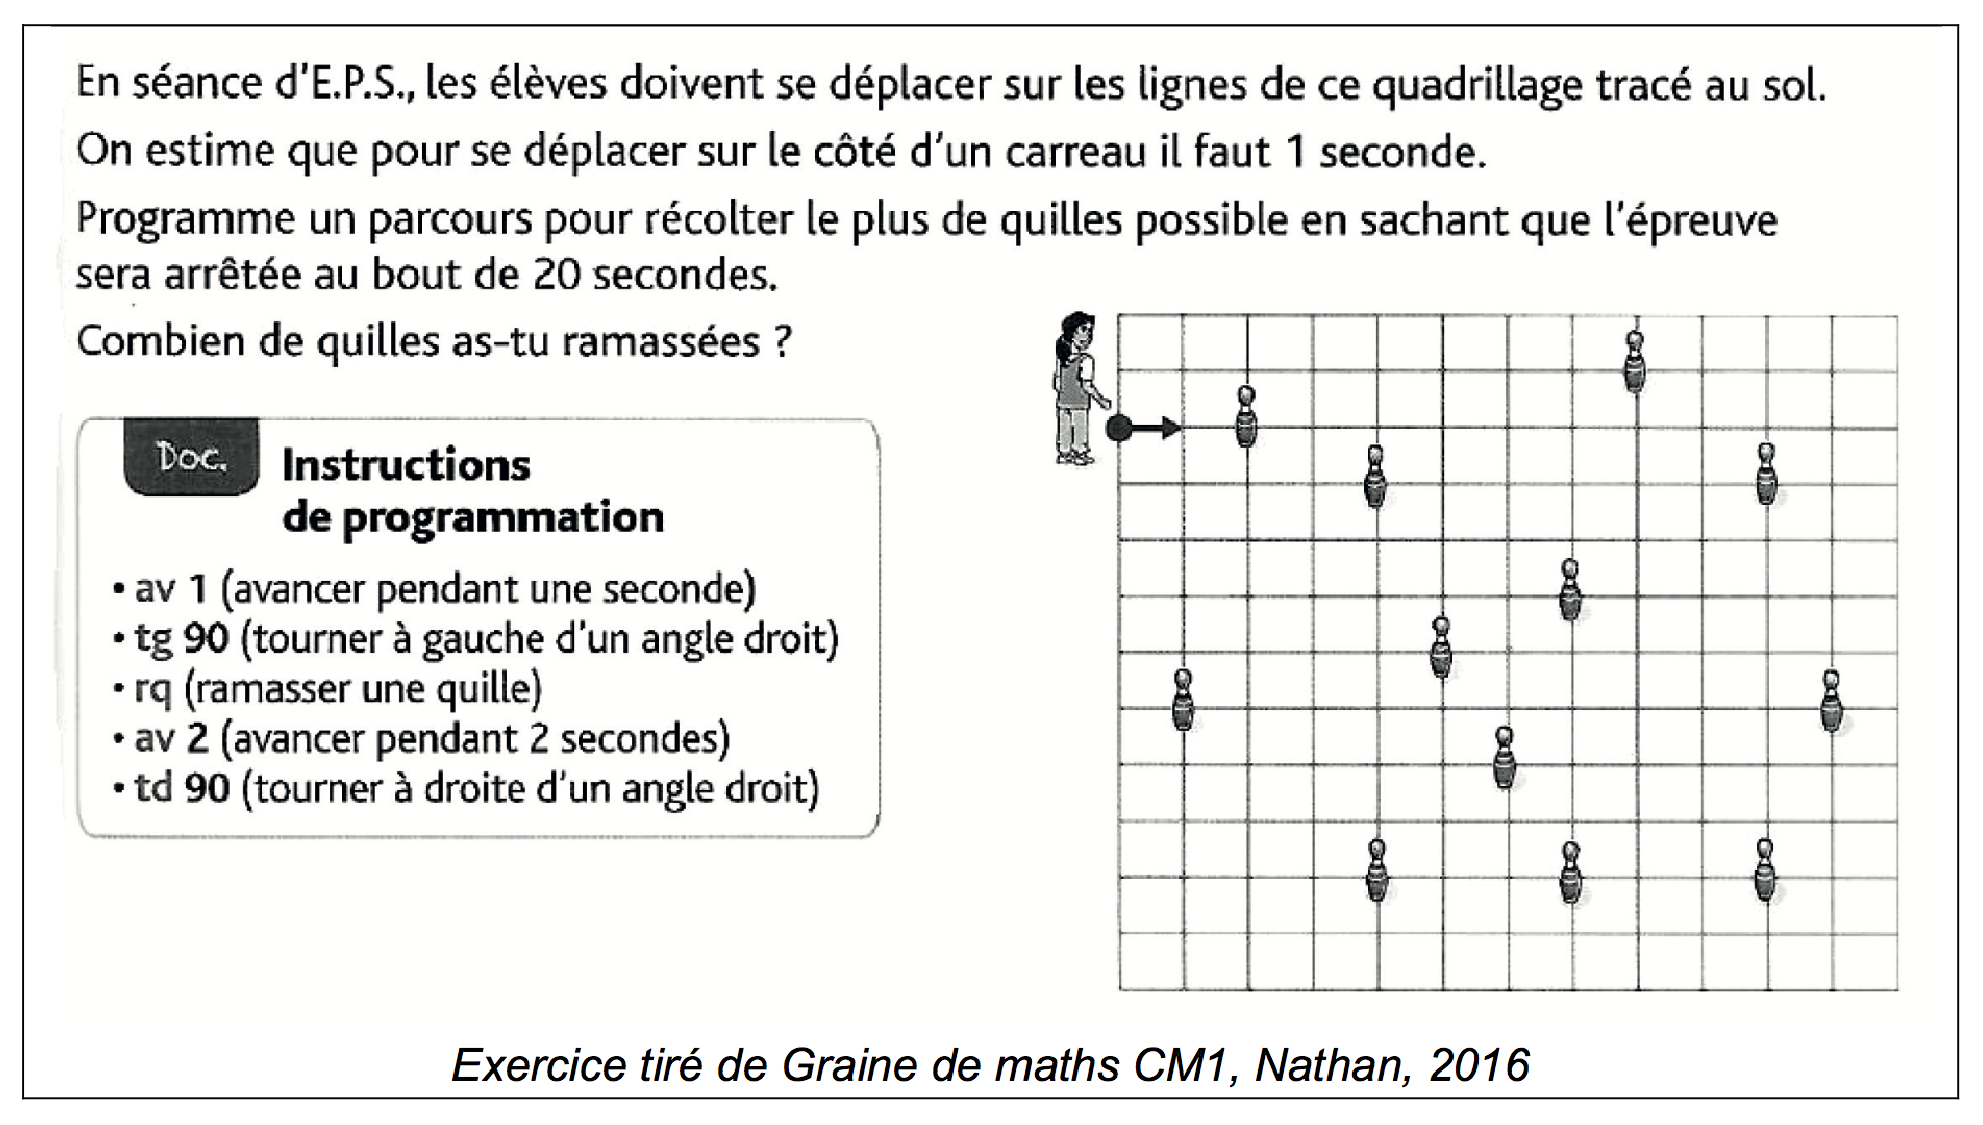
\includegraphics[width=12cm]{Geometrie_did/Images/Geo6_analyse_programmation}
\end{center}

\begin{enumerate}
   \item Citer deux connaissances ou savoir-faire mathématiques nécessaires à la réussite de cet exercice.
   \item Utiliser les deux productions d’élèves reproduites ci-après pour répondre aux questions ci-dessous.
   \begin{enumerate}
      \item Analyser chaque production en termes de réussites et d’erreurs
      \item Proposer deux dispositifs de remédiation que l’enseignant pourrait mettre en œuvre à l’attention d’Oriane.
   \end{enumerate}
\end{enumerate}

\begin{center}
   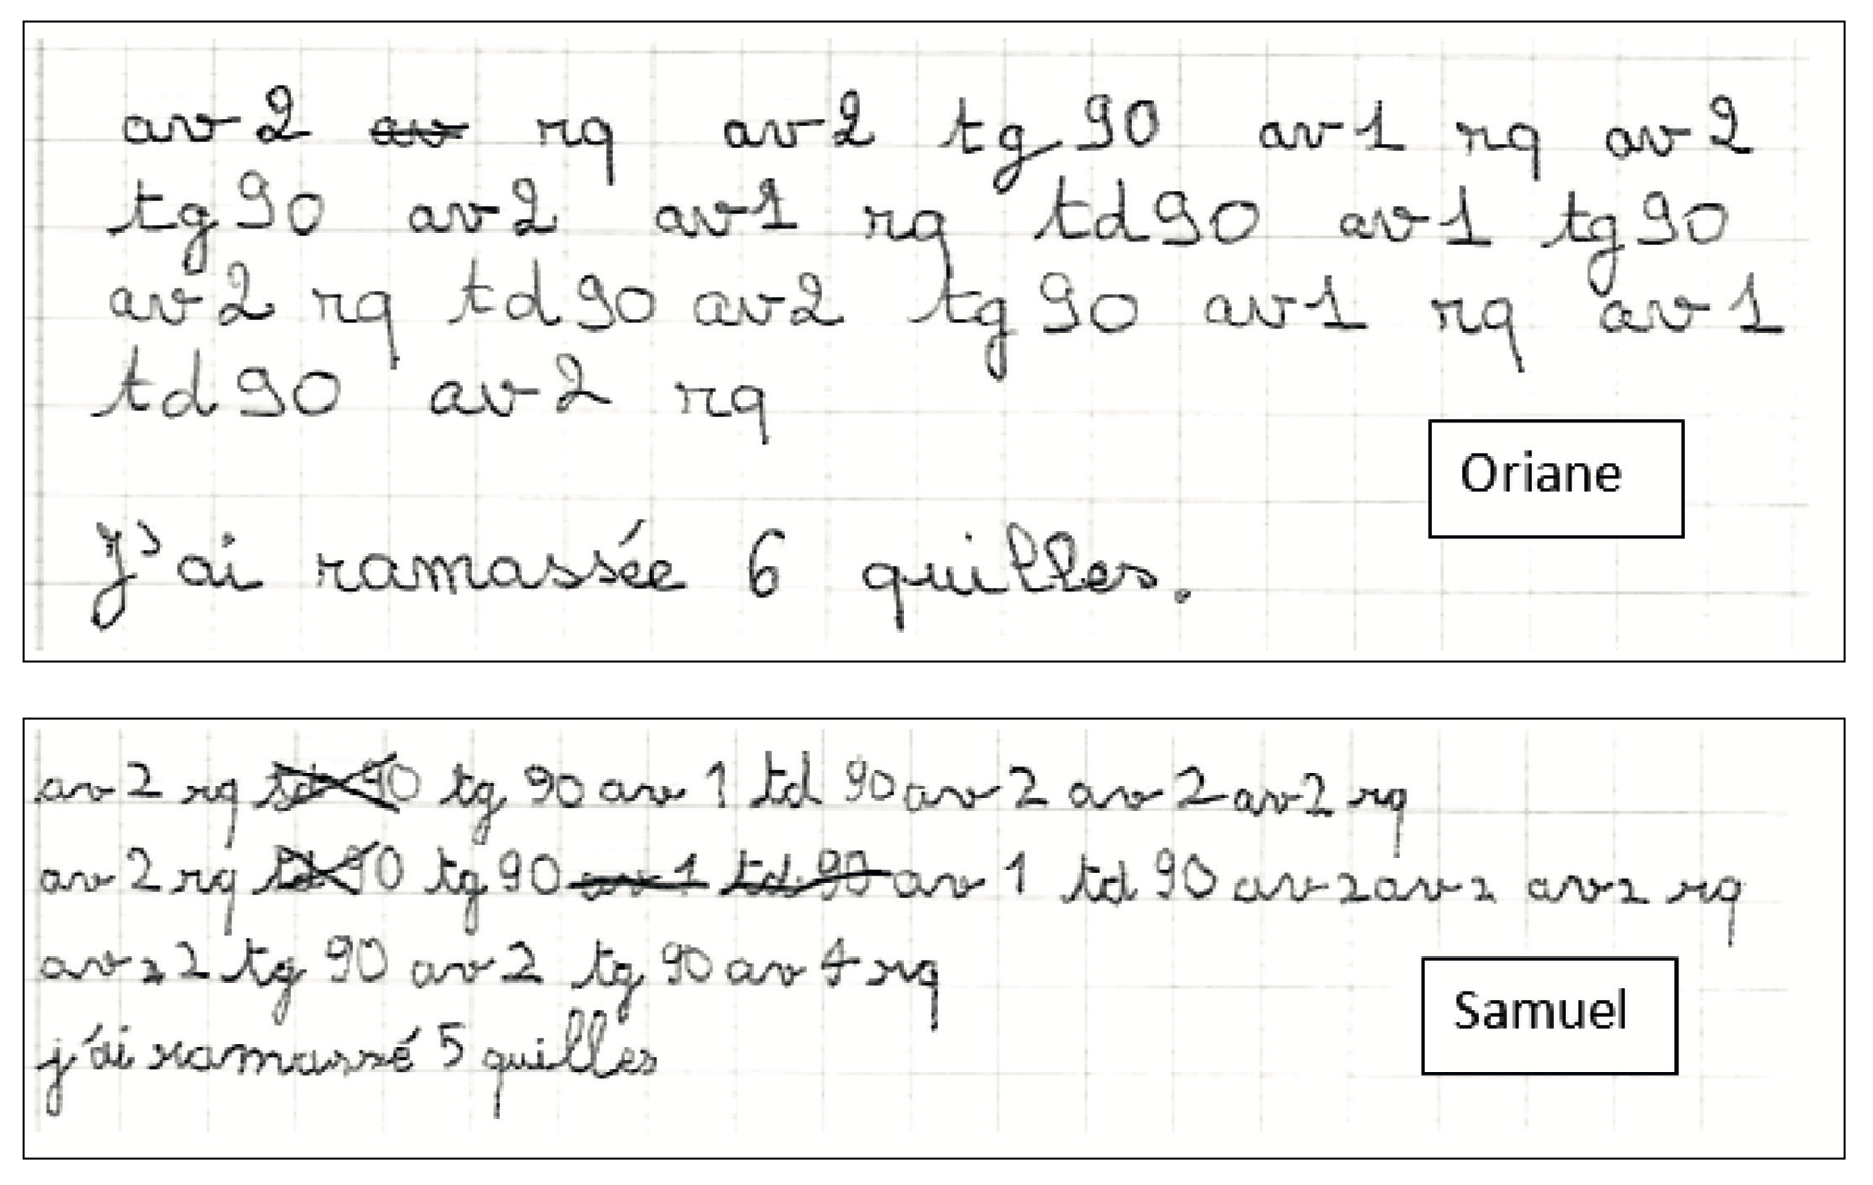
\includegraphics[width=12cm]{Geometrie_did/Images/Geo6_analyse_programmation_eleves}
\end{center}
\end{exercice}

\begin{corrige}
\ \\ [-5mm]
\begin{enumerate}
   \item \textcolor{A2}{$\bullet$} programmer le déplacement d’un personnage sur un plan ;
   \begin{itemize}
      \item se repérer dans l'espace ;
      \item résoudre un problème utilisant un repérage de l'espace.
   \end{itemize}
   \item 
   \begin{enumerate}
      \item {\bf Oriane} : elle a trouvé 6 quilles ce qui est le maximum de quilles possibles de récupérer en 20 secondes. Son chemin semble correct dans sa tête, cohérent au niveau des instructions \og av \fg{}, \og rq \fg{} et le temps de 20 secondes est respecté mais les instructions d'orientation (droite et gauche) sont souvent fausses. \\
      {\bf Samuel} : il donne un premier programme juste permettant de récupérer 2 quilles (ligne 1). Il maîtrise sur cet exemple les diverses instructions de déplacement et d'orientation. Il semble ensuite qu'il recommence du point de départ et construit son déplacement sans anticipation, ce qui lui donne in fine le même parcours que précédemment. Enfin, il tente un troisième parcours pour lequel on ne sait pas vraiment d'où il part ni ce qu'il fait. Il a utilisé plus de 20 déplacements et une nouvelle instruction : \og av4 \fg.
      \item {\bf Oriane} a des difficultés d'orientation : elle mélange les repérages absolus et relatifs, c'est donc vers cette remédiation qu'il faut se tourner, on peut lui proposer par exemple :
      \begin{itemize}
         \item une activité déconnectée réelle en lui faisant faire les déplacements de manière effective sur sur un grand quadrillage dans la cours de l'école (jeu du robot idiot) ; 
        \item une activité sur ordinateur ou tablette afin de percevoir l'effet d'une erreur d'instruction en direct (ScratchJr, Scratch, Lightbot, Gcompris labyrinthe\dots).
     \end{itemize}
     {\bf Samuel} semble avoir des difficultés d'anticipation, on peut lui proposer de tracer le déplacement qu'il souhaite obtenir sur le quadrillage, puis de coder ce déplacement tout en dénombrant le temps écoulé et le nombre de quilles récupérées.
   \end{enumerate}
\end{enumerate}
\end{corrige}



%%%%%%%%%
\Recreation %%%
%%%%%%%%%


\setcounter{exercice}{0}

\begin{exercice*}[\fbox{C1} - Les abaques] %%%%%%%%%%%%

{\bf Objectifs et compétences}
   \begin{itemize}
      \item Comprendre la notion de modèle à reproduire.
      \item Respecter un ordre vertical (les pièces à disposer étant soumis à la pesanteur) avec un modèle horizontal.
      \item Reconnaître des couleurs.
      \item Développer des compétences langagière par un vocabulaire précis : au dessus, en dessous.
      \item Ranger des objets selon leur couleur.
      \item Résoudre un problème simple. \medskip
   \end{itemize}

{\bf Le matériel}
\begin{center}
   \begin{tabular}{C{4.5}|C{4.5}|C{4.5}}
      Des abaques à 3 ou 4 tiges & Des pièces percées à insérer & Des cartes modèles \\
      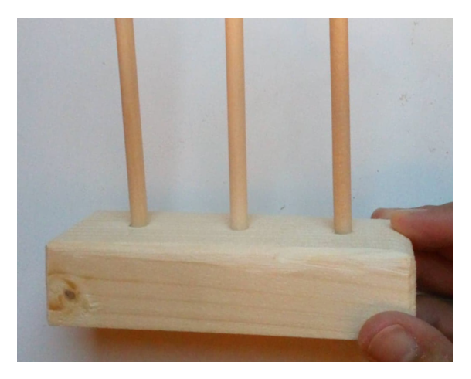
\includegraphics[width=4cm]{Geometrie_did/Images/Geo6_activites_abaques_tiges1}
      &
      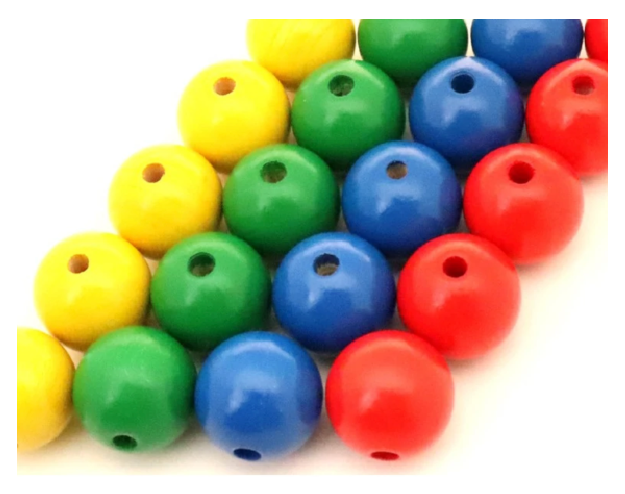
\includegraphics[width=4cm]{Geometrie_did/Images/Geo6_activites_abaques_tiges2}
      &
      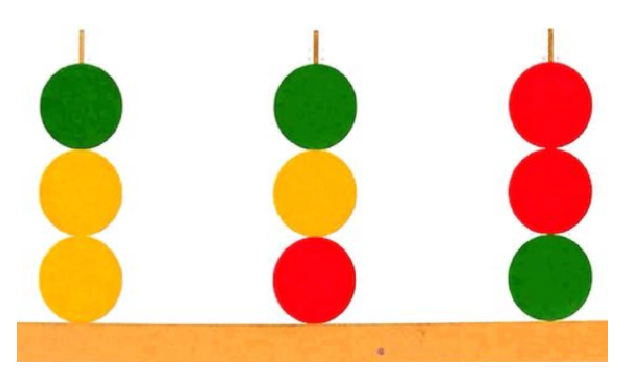
\includegraphics[width=4.5cm]{Geometrie_did/Images/Geo6_activites_abaques_tiges3}
      \\
   \end{tabular} \\
\end{center}

{\bf Déroulement de l'activité} \\
Les élèves sont en atelier dirigé par groupe de deux : il y a un acteur et un observateur. \\
L'enseignant donne une carte modèle, un abaque et neuf pièces à chaque joueur et explique le but à atteindre. Les cartes modèles sont présentées avec le trait horizontal en bas de façon à ressembler à l'abaque. \\
Quand un joueur pense avoir réalisé une copie conforme au modèle, il demande l’avis de son observateur. Si lies deux enfants sont d'accord, l'enseignant valide ou non avec eux puis les rôles sont inversés et les enfants prennent une autre carte modèle. \\
Lorsque les enfants ont bien compris en quoi consiste ta tâche, l'atelier devient autonome : les enfants viennent chercher eux-mêmes de nouvelles cartes modèles. \medskip

{\bf Variables} \\
-- Varier les couleurs. \\
-- Varier le nombre de tiges. \\
-- Varier le nombre d'objets à insérer. \\
-- Faire le travail inverse : proposer un abaque plein et demander aux élèves de colorier une carte vierge.

\begin{center}
   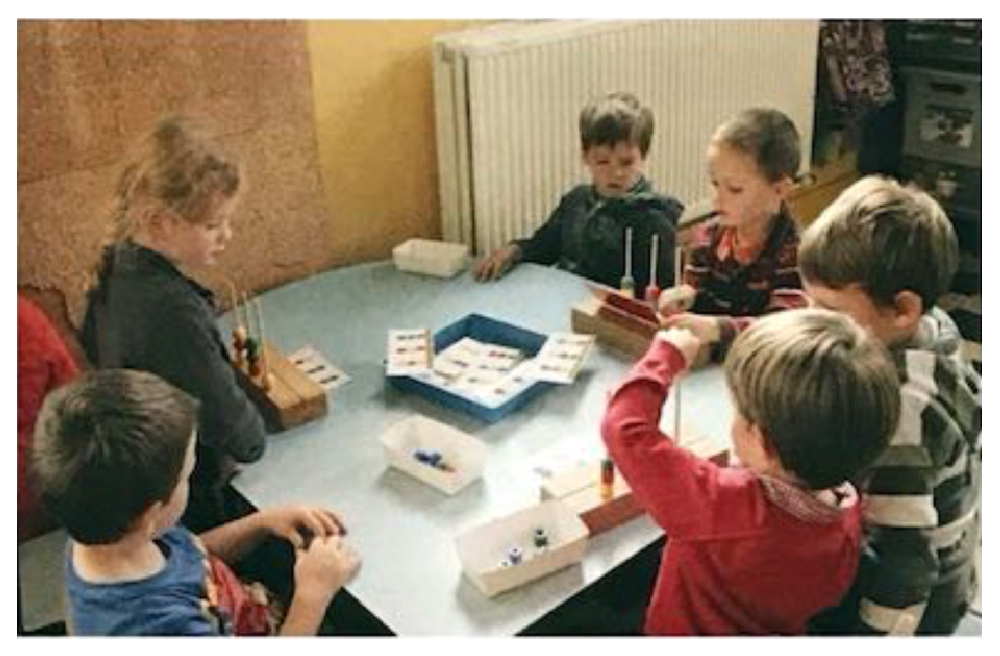
\includegraphics[width=8.25cm]{Geometrie_did/Images/Geo6_activites_abaques_tiges4}
\end{center}

\hfill{\it\small Source. Découvrir les maths MS : Abaques p. 34-46.}
\end{exercice*}


\begin{exercice*}[\fbox{C1} - Les abaques taquins] %%%%%

{\bf Objectifs et compétences}
   \begin{itemize}
      \item Développer des compétences langagière par un vocabulaire précis : au dessus, en dessous, entre, boule supérieure/inférieure, déplacement.
      \item Organiser des actions pour atteindre un but.
      \item Observer et analyser des organisations spatiales dans le micro-espace.
      \item Résoudre une situation-problème complexe. \medskip
   \end{itemize}

{\bf Le matériel}
\begin{center}
   \begin{tabular}{C{4.5}|C{4.5}|C{4.5}}
      Des abaques à 3 tiges & Des cartes modèles & Une feuille de route \\
      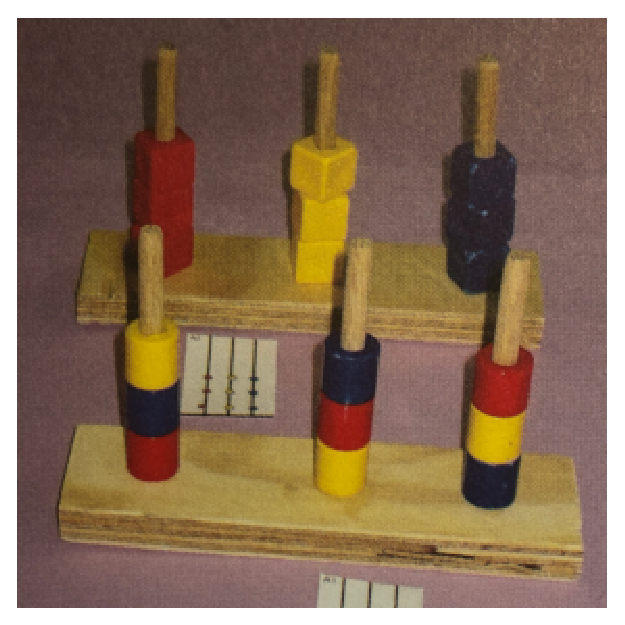
\includegraphics[width=4cm,height=3.5cm]{Geometrie_did/Images/Geo6_activites_abaques_taquins1}
      &
      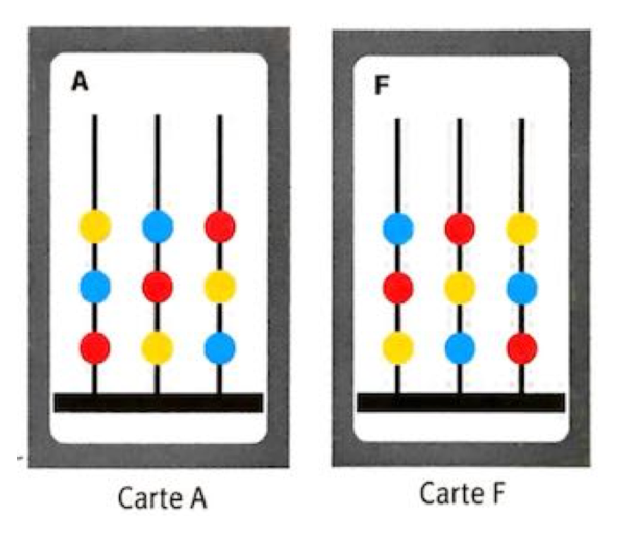
\includegraphics[width=4cm]{Geometrie_did/Images/Geo6_activites_abaques_taquins2}
      &
      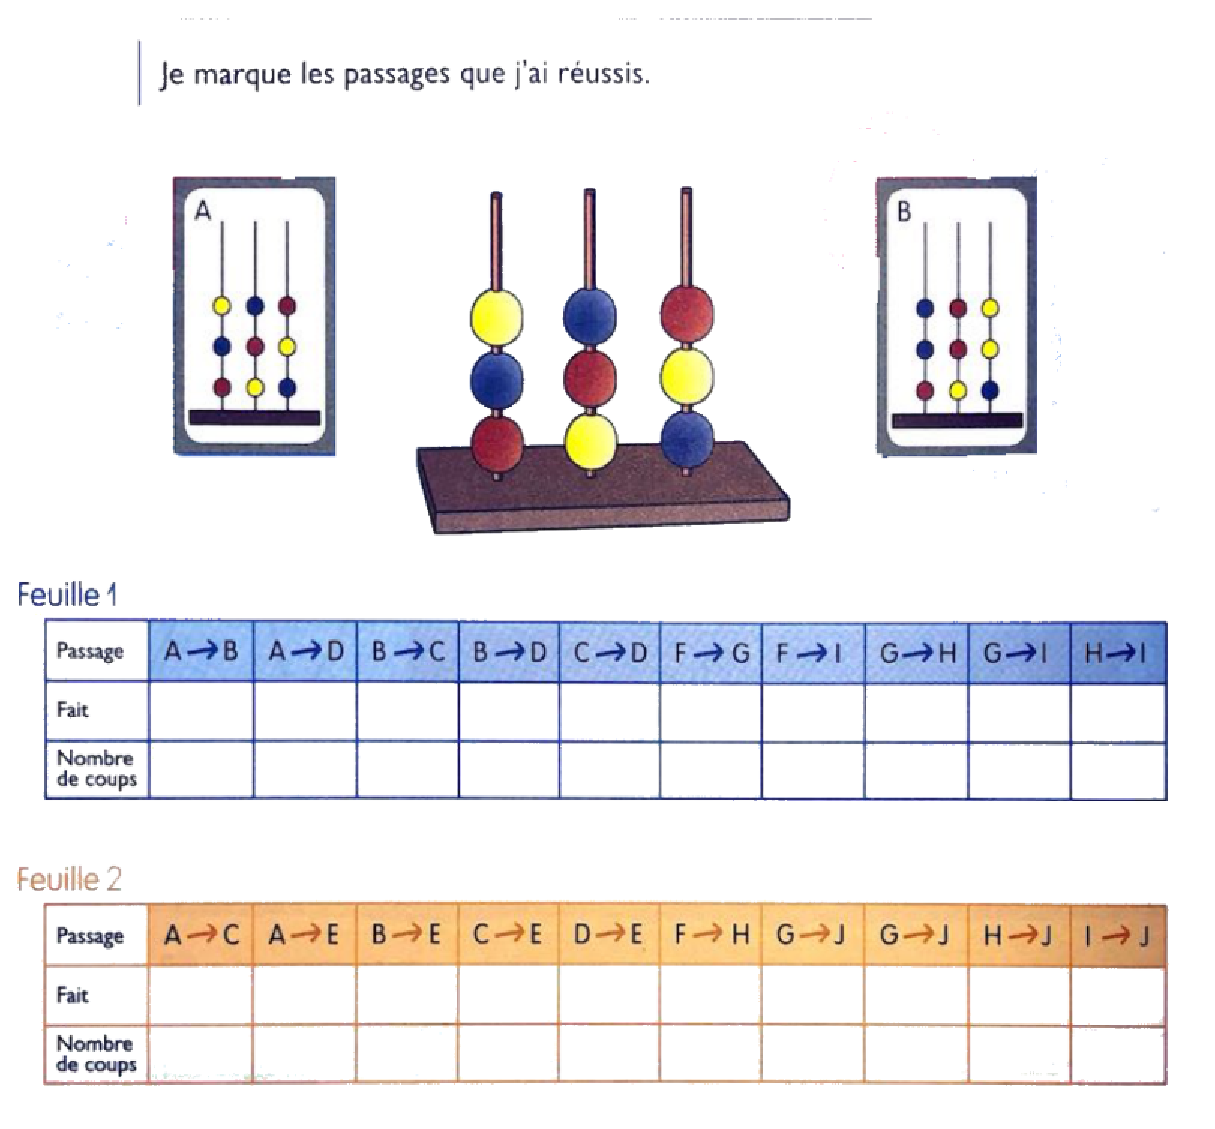
\includegraphics[width=4cm]{Geometrie_did/Images/Geo6_activites_abaques_taquins3}
      \\
   \end{tabular} \\
\end{center}

{\bf Déroulement de l'activité} \\
Les élèves sont en atelier dirigé. \\
L'enseignant explique aux enfants le principe du jeu des abaques : \og Vous devez prendre la carte A (carte de départ) et placer les boules sur l'abaque comme sur cette carte \fg. \\
À partir de la position des boules de la carte A, il faudra mettre les boules comme sur la carte F (carte d’arrivée) en respectant certaines règles :
\begin{itemize}
   \item Seule la boule supérieure d'une tige peut être retirée et placée sur une autre tige, mais il ne faut pas dépasser 5 boules sur une même tige.
   \item Aucune boule ne peut rester hors des tiges (dans la main d'un joueur, par exemple).
   \item Une même boule peut être déplacée plusieurs fois.
\end{itemize}
La recherche est individuelle. Dans un second temps, un observateur peut être désigné pour compter le nombre de déplacements qui ont été nécessaires pour passer d'une carte à l'autre. \\
Les \og problèmes \fg{} à chercher sont définis par l’enseignant.e. Le choix des cartes mises en relation est important car le passage de l’une à l’autre ne représente pas la même difficulté (voit tableau ci-dessous). \\ [5mm]
\begin{minipage}{10cm}
   \begin{tabular}{|*{11}{c|}}
      \hline
      & A & B & C & D & E & F & G & H & I & J \\
      \hline
      A & & 11 & 5 & 11 & 8 & 18 & 24 & 21 & 24 & 19 \\
      \hline
      B & 11 & & 10 & 11 & 6 & 18 & 18 & 19 & 21 & 22 \\
      \hline
      C & 5 & 10 & & 11 & 6 & 19 & 24 & 24 & 22 & 19 \\
      \hline
      D & 11 & 11 & 11 & & 8 & 17 & 18 & 18 & 17 & 18 \\
      \hline
      E & 8 & 6 & 6 & 8 & & 18 & 22 & 16 & 23 & 19 \\
      \hline
      F & 18 & 18 & 19 & 17 & 18 & & 11 & 5 & 11 & 8 \\
      \hline
      G & 24 & 18 & 24 & 18 & 22 & 11 & & 10 & 11 & 6 \\
      \hline
      H & 21 & 19 & 24 & 18 & 16 & 5 & 10 & & 11 & 6 \\
      \hline
      I & 24 & 21 & 22 & 17 & 23 & 11 & 11 & 11 & & 8 \\
      \hline
      J & 19 & 22 & 19 & 18 & 19 & 6 & 6 & 6 & 8 & \\
      \hline
   \end{tabular}
\end{minipage}
\begin{minipage}{6cm}
   Les élèves ont une feuille de route où ils peuvent cocher les problèmes résolus.
   \begin{itemize}
      \item Niveau 1 : de 5 à 8 déplacements.
      \item Niveau 2 : de 10 à 15 déplacements.
      \item Niveau 3 : de 16 à 20 déplacements.
      \item Niveau 20 : plus de 20 déplacements. \\
   \end{itemize}
   \vfill\hfill{\it\small Source. Découvrir les maths GS : Abaques taquins p. 68-70}
\end{minipage}
\end{exercice*}


\begin{exercice*}[\fbox{C1} - Les 5 tours alignées]
Cette situation aborde les trois aspects numérique (cardinal et ordinal), géométrique et logique. \\

{\bf Objectifs et compétences}
   \begin{itemize}
      \item Prendre conscience qu’un objet plus grand qu’un autre peut cacher ce dernier. 
      \item Utiliser des informations numériques dans un cadre spatial.
      \item Prendre en compte deux contraintes.
      \item Développer des compétences langagière par un vocabulaire précis : devant, derrière, dessus, en face, caché, extrémité, au bout, à gauche, à droite.
      \item Résoudre un problème simple. \medskip
   \end{itemize}

\partie[construire 5 tours dans le méso-espace et s'approprier l'idée de \og point de vue \fg] %%%

{\bf Le matériel :}
\begin{center}
   \begin{tabular}{C{4}|C{5.5}|C{3.5}}
      5 tours de 1 à 5 étages & Un banc pour y déposer les tours & \\
      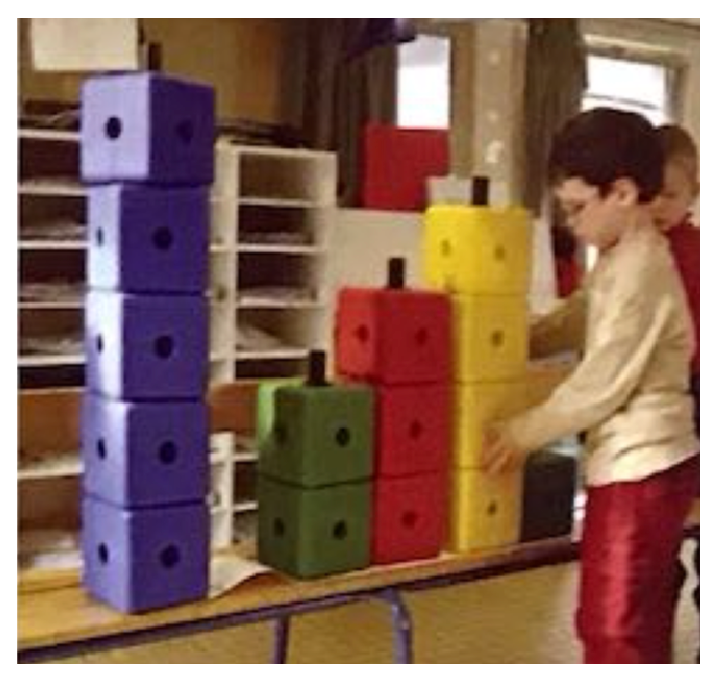
\includegraphics[width=4cm]{Geometrie_did/Images/Geo6_activites_tours1}
      &
     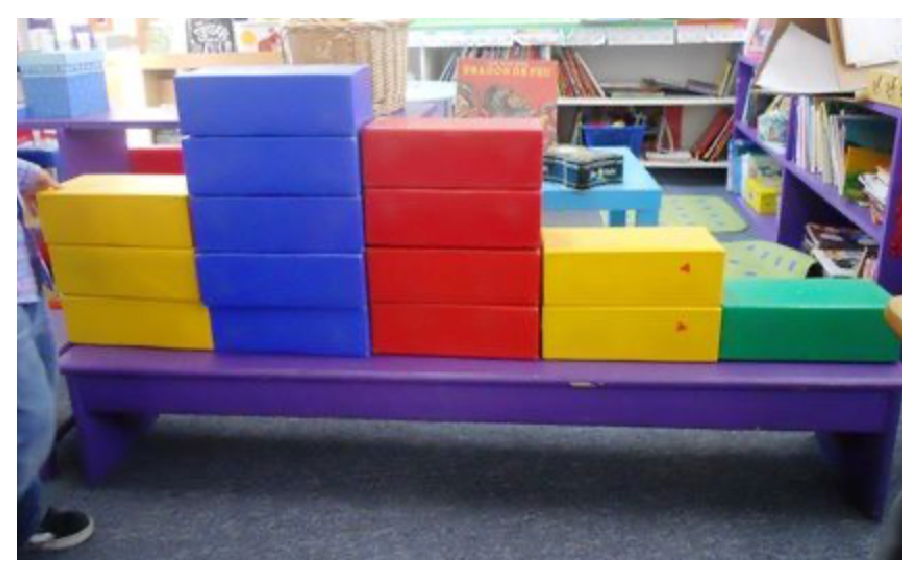
\includegraphics[width=5.5cm]{Geometrie_did/Images/Geo6_activites_tours2}
      &
      \begin{minipage}[b]{3.5cm}
         Une bande de papier de 7 cases de même mesure que la base des tours. \\ [5mm]
         \fbox{\white \,0\,}\fbox{\white \,0\,}\fbox{\white \,0\,}\fbox{\white \,0\,}\fbox{\white \,0\,}\fbox{\white \,0\,}\fbox{\white \,0\,} \\ [3mm]
      \end{minipage}
      \\
   \end{tabular} \\
\end{center}

\begin{description}
   \item[Étape 1:] présenter les 5 tours. \\
   Les enfants et les tours ont des tailles de même ordre. \\
   Le matériel est montré aux enfants : \og J’ai fabriqué des tours avec les cubes/pavés/boites. Comment sont-elles ? \fg. Les enfants décrivent ces tours avec leurs mots et l’enseignant.e énonce finalement : \og il y a une tour bleue de 5 étages, une tour rouge de 3 étages\dots \fg.
   \item[Étape 2:] s’approprier l’idée de point de vue. \\
   L’enseignant.e aligne ensuite les 5 tours sur la grande bande de papier. Par exemple, la disposition des tours peut-être la suivante (figure de droite) : \fbox{\white \huge\,0\,}\fbox{\huge\,3\,}\fbox{\huge\,5\,}\fbox{\huge\,4\,}\fbox{\huge\,2\,}\fbox{\huge\,1\,}\fbox{\white\huge\,0\,} \\
   Les enfants sont invités, un à un, à se déplacer autour du matériel et à dire ce qu’ils voient. Cette étape doit leur permettre de découvrir d'abord qu’un ensemble d’objets n’est pas vu de la même façon suivant l’endroit d'où on l'observe. Dans un deuxième temps, il s’agit de comprendre et de dire à quelles conditions un objet peut en cacher un autre.
   \item[Étape 3:] combien voit-on de tours à chaque extrémité ? \\
   L'enseignant.e demande à chaque enfant de déterminer combien il voit de tours à chaque extrémité. Les enfants se déplacent, tournent autour de l'assemblage et on précise le vocabulaire retenu : \og les tours, les étages \fg. Par exemple, dans le problème précédent, les tours qui seront vues à chaque extrémité sont : au nombre de 2 d'un côté, la tour 5 cachant les 3 autres tours ; au nombre de 4 de l'autre côté. Ces nombres sont donnés oralement. On peut résumer en plaçant des étiquettes aux extrémités de la bande :
   \begin{center}
      \fbox{\red\huge\,2\,}\fbox{\huge\,3\,}\fbox{\huge\,5\,}\fbox{\huge\,4\,}\fbox{\huge\,2\,}\fbox{\huge\,1\,}\fbox{\red\huge\,4\,}
   \end{center}
Plusieurs dispositions différentes des tours sont ainsi proposées aux enfants.
\end{description}


\partie[résoudre des problèmes dans le méso-, puis dans le micro-espace]
{\bf Le matériel}
\begin{itemize}
   \item Le même matériel que dans la partie A.
   \item Des étiquettes rouges et noires numérotées de 1 à 5.
   \item Des bandes de 7 cases vierges de petit format (14 cm par 2 cm par exemple). \smallskip
\end{itemize}

\begin{description}
   \item[Étape 1:] en vraie grandeur, avec les gros cubes/pavés. \\
   Les enfants sont devant la grande bande de papier de 7 cases et l’enseignant.e explique ce qu’il attend : deux élèves se placent chacun à l'une des extrémités. Un autre élève doit placer les tours sur la table en respectant deux contraintes : par exemple, on doit voir à l'une des extrémités 1 tour, et à l'autre 4 tours. La solution est ajustée si nécessaire, par essais successifs. \smallskip
   \begin{center}
      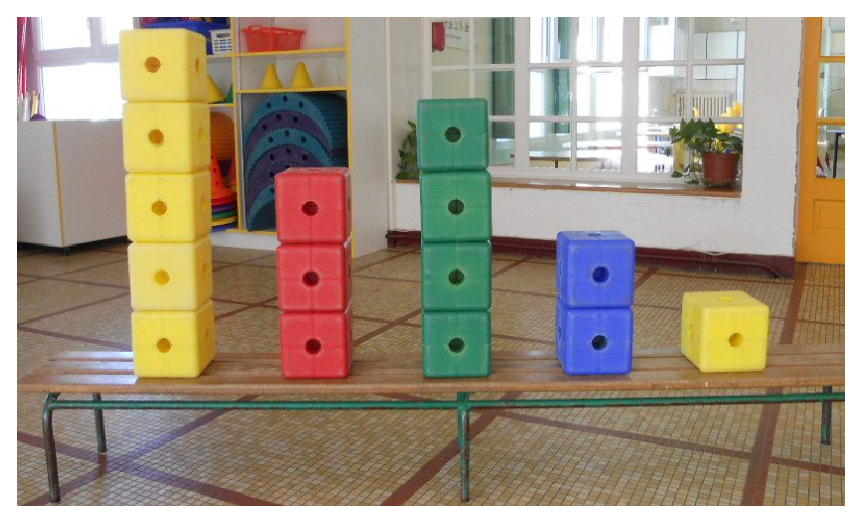
\includegraphics[height=3.5cm]{Geometrie_did/Images/Geo6_activites_tours3} \qquad 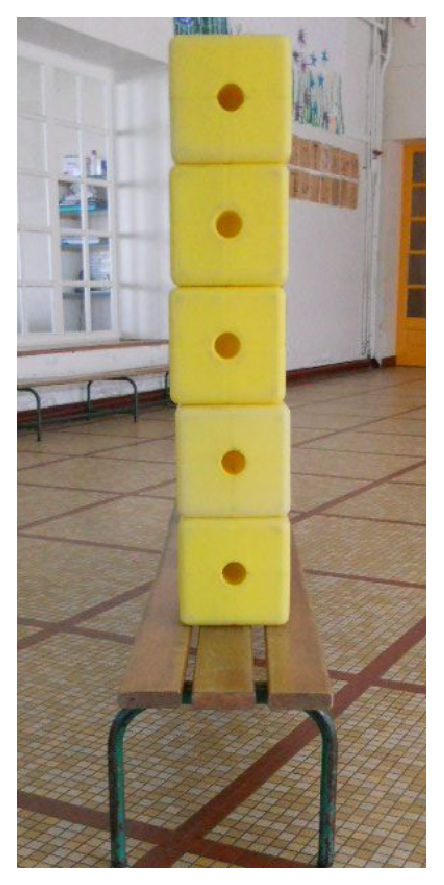
\includegraphics[height=3.5cm]{Geometrie_did/Images/Geo6_activites_tours5} \qquad 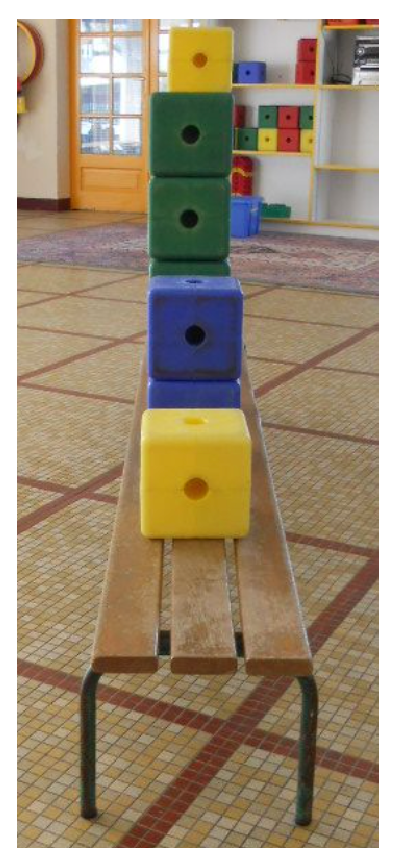
\includegraphics[height=3.5cm]{Geometrie_did/Images/Geo6_activites_tours4}
   \end{center}
   Plusieurs problèmes sont ainsi proposés aux enfants, puis on passe à la verbalisation : les élèves expliquent ce qu'ils ont pu constater. Par exemple, le 1 oblige à mettre la tour 5, c’est-à-dire la plus grande, au premier plan puisqu'elle doit cacher toutes les autres tours. Le 5 implique que les tours doivent être placées par ordre croissant depuis la position de l’observateur. Il est tout à fait possible d'utiliser les étiquettes nombres rouges correspondant au nombre de tours à chaque extrémité si besoin. \\
   Le solution n'est pas nécessairement unique, et certaines configurations n'ont pas de solution : il s'agit de (1,1) ; (2,5) ; (3,4) ; (3,5) ; (4,5) ; (5,5).
   \item[Étape 2] : schématisation du problème dans l’espace à deux dimensions. \\
   Les élèves schématisent la solution trouvée et toujours visible sur les grandes bandes en plaçant les étiquettes numérotées : l'objectif est de comprendre la schématisation des vraies tours par des étiquettes nombres, dans un espace de même dimension. \\
   L'enseignant.e positionne sur la bande support, les étiquettes nombres rouges et précise ce qui est attendu, par exemple : \og Les nombres rouges 1 et  4 que j’ai placés, c’est pour rappeler qu’ici on devait voir une seule tour et que là on devait en voir quatre \fg. \\
   Les enfants ont à leur disposition 5 étiquettes nombres noires qui représentent les tours à partir de leur nombre d'étages et ils les positionnent sur la bande, comme ils ont placé les tours en vraie grandeur. Il ne s’agit pas, ici, de résoudre le problème dans l'espace à 2 dimensions, mais seulement de conserver la trace de la résolution qui vient d'être faite en vraie grandeur.
   \begin{center}
      \fbox{\red\huge\,1\,}\fbox{\huge \,5\,}\fbox{\huge\,3\,}\fbox{\huge4}\fbox{\huge\,2\,}\fbox{\huge\,1\,}\fbox{\red\huge\,4\,} 
   \end{center}
   La grande bande précédente est alors cachée et l'enseignant.e distribue à chaque enfant une bande problème identique, mais en plus petit (les cases ne font que 2 cm de côté). Chaque enfant écrit les nombre correspondants aux noms de chaque tour à la bonne place sur la bande problème : c'est la trace écrite individuelle du positionnement des tours.
   \begin{center}
      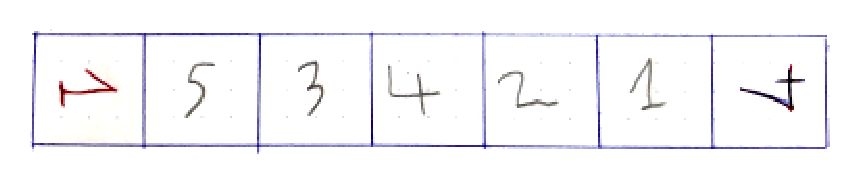
\includegraphics[height=1.05cm]{Geometrie_did/Images/Geo6_activites_tours6}
   \end{center}
\end{description}

\partie[résolution individuelle dans le micro-espace]
{\bf Le matériel}
\begin{center}
   \begin{tabular}{C{4.5}|C{4.5}|C{4.5}}
      Des tours de 1 à 5 étages & Une ou deux figurines & Des bandes problèmes \\
      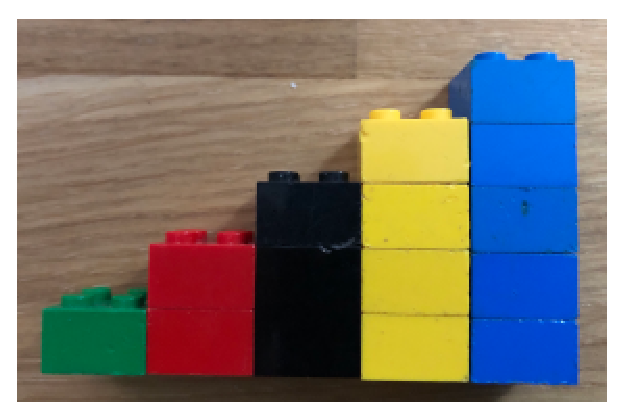
\includegraphics[width=4cm]{Geometrie_did/Images/Geo6_activites_tours7}
      &
      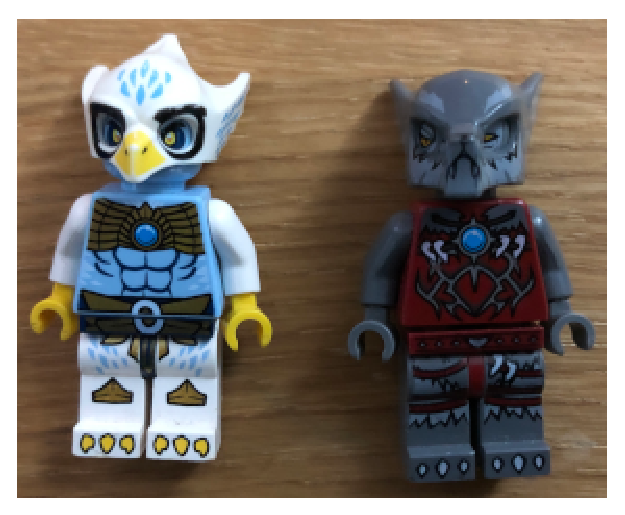
\includegraphics[width=3.2cm]{Geometrie_did/Images/Geo6_activites_tours8}
      &
      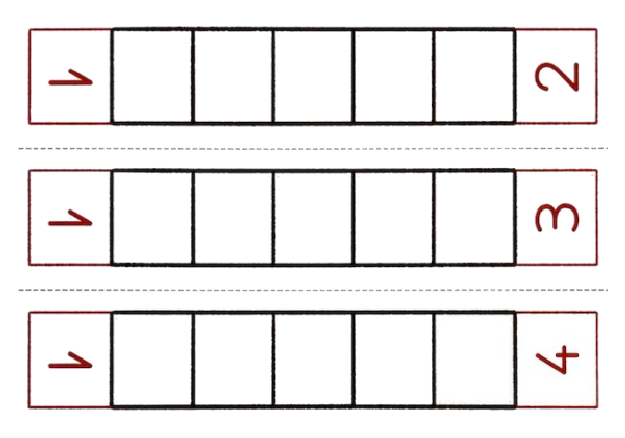
\includegraphics[width=4cm]{Geometrie_did/Images/Geo6_activites_tours9}
      \\
   \end{tabular} \\
\end{center}

   C'est un approfondissement de la phase précédente. Les problèmes sont maintenant posés dans l'espace de la feuille de papier. \\
   L'enseignant.e explique que l'on va faire \og la même chose, mais en plus petit \fg. Il précise, en particulier, le rôle des personnages fictifs : \og Maintenant, c’est le petit personnage qui regarde les tours et vous, vous allez poser les petites tours pour que le personnage voie juste le nombre de tours indiqué sur les étiquettes rouges \fg. \\
   Puis il présente les petites tours : \og Elles sont comme les grandes avec lesquelles vous avez joué sur les tables : celle-ci a deux étages, c'est la tour 2. Qui peut montrer la tour 5 ?, etc. \fg. \\
   Enfin, il montre une bande problème : \og Par exemple, ici, le petit personnage doit voir 4 tours de ce côté et 2 tours de l’autre côté \fg
   \begin{center}
      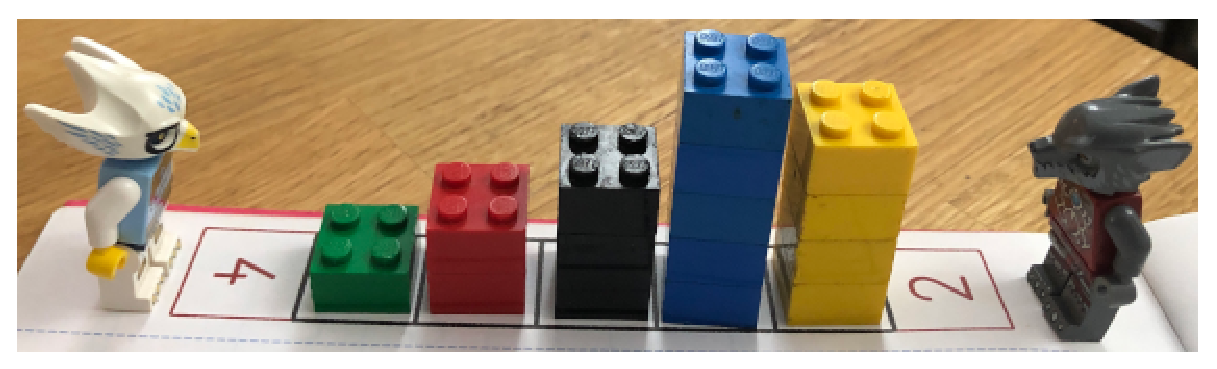
\includegraphics[width=10cm]{Geometrie_did/Images/Geo6_activites_tours10}
   \end{center}
   Lorsque l'élève aura posé les tours sur la bande et bien vérifié que le petit personnage voit bien le nombre de tours qui est marqué à chaque extrémité, il enleve chaque tour une par une et écrit à la place le nombre qui convient. \\
   La validation se fait par échange des productions entre les enfants, en présence de l’enseignant : en cas d'erreur, l'enfant est invité à positionner à nouveau les tours. \\

Cette activité peut être poursuivie en GS par l'activité des 9 tours sur quadrillage (découvrir les maths GS p. 144-150), voire des 16 tours.
   \begin{center}
      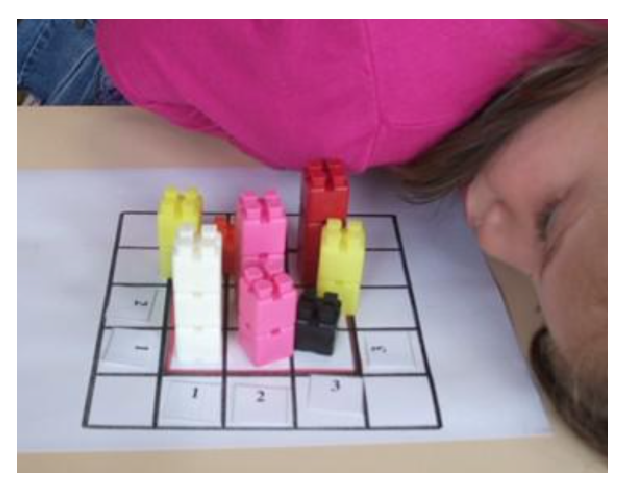
\includegraphics[height=5cm]{Geometrie_did/Images/Geo6_analyse_quadrillage1} \qquad  \includegraphics[height=5cm]{Geometrie_did/Images/Geo6_analyse_quadrillage2}
   \end{center}

   \vfill\hfill{\it\small Source. Découvrir les maths : 5 tours alignées p. 151-157 (MS) et p. 74-79 (GS)}
\end{exercice*}

\pagebreak


\begin{exercice*}[\fbox{C1} - Exemples d'activités avec les Kubix]
\begin{description}
   \item[Le château.] Activités à partir de construction de châteaux.
      \begin{itemize}
         \item {\bf Réalisation de figures libres.} Première catégorisations à partir des réalisations des élèves.
         \begin{center}
            \includegraphics[width=7cm]{Geometrie_did/Images/Geo6_activites_chateau5}
         \end{center}
         \item {\bf Construire un château plus haut} que celui de la maîtresse, un objet de la classe\dots{} Verbalisation à partir des réalisations : pièces les plus ou les moins utilisées, pièce en haut de la construction, pièces non utilisées\dots
         \item {\bf Construction d’un château collectif} en utilisant tout le matériel proposé. Les sphères agiront comme intrus et seront mises de côté. Permet de dégager les propriétés des solides : sont-ils stable ou non, la notion d’arrête, de face.
         \begin{center}
            \includegraphics[width=8cm]{Geometrie_did/Images/Geo6_activites_chateau3}
         \end{center}
         \item {\bf Associer points de vue et solides :} retrouver les photographies prises de différents points de vue correspondantes à un assemblage de solides donné. \\
         Variables : complexité de la figure de départ, présence d’un intrus, nombre de solides photographiés, comparaison possible ou non avec la construction.
         \item {\bf Reproduire un château} : avec un modèle proche, réel ou en photo, avec un modèle éloigné, en limitant le nombre de déplacements, sous la dictée d’un camarade, par un système de commandes, grâce à la représentation faite par un camarade.
      \end{itemize}
      \begin{center}
         \includegraphics[width=4cm]{Geometrie_did/Images/Geo6_activites_chateau1}\qquad \qquad \includegraphics[width=4.5cm]{Geometrie_did/Images/Geo6_activites_chateau2}
      \end{center}
   \item[Le jeu de Kim.]Les jeux de KIM sont des jeux traditionnels créés à partir d’un livre de Rudyard Kipling : Kim (Kimball O’Hara) est un orphelin, fils d’un ancien soldat, qui survit comme il peut. Sa seule certitude est qu’un jour \og un grand taureau rouge sur un champ vert, avec le colonel sur son grand cheval et neuf cents diables \fg{} viendront le chercher. Il part donc à l’aventure et sera successivement messager puis agent secret des services britanniques. Il s’entraînera à observer les moindres détails de son environnement pour en informer ses supérieurs\dots
      \begin{itemize}
         \item {\bf Kim touché} : on dispose d'un sac géant contenant tous les solides, qui ne sont pas visibles. Sortir le même que celui qui est montré (PS), que celui qui est demandé (MS), que celui dont on présente la carte d’identité.
         \item {\bf Kim vue caché} : déposer 5 des solides sur la table, les enfants observent les objets pendant environ 2 min. Le meneur de jeu recouvre ensuite les objets avec un tissu et les joueurs doivent dire tous les objets, sans en oublier.
         \item {\bf Kim vue ajouté/retiré} : 5 objets sont déjà posés sur la table. Après observation les élèves ferment les yeux et le meneur  ajoute/retire un objet. Quel est cet objet ?
         \item {\bf Kim vue déplacé} : 5 objets sont déjà posés sur la table. Après observation les élèves ferment les yeux et le meneur   déplace un objet. Quel est cet objet ?
      \end{itemize}
   \item[Le Tri sélectif.] Proposer un grand nombre de solides à trier et faire émerger les critères de classement et de tri : nombre de faces, roule ou non, tient sur une face\dots
   \item[Les empreintes.]À faire par exemple avec de la pâte à modeler, le contour des figures\dots
      \begin{itemize}
         \item Chercher des objets, des formes, qui correspondent à une empreinte donnée sur une feuille. Variable : placer les formes loin des empreintes.
         \item Construire des empreintes à partir d’une forme (peinture, pâte à modeler, contour\dots). Puis demander le maximum d’empreintes différentes, autant d’empreintes que de faces.
         \begin{center}
            \includegraphics[width=6cm]{Geometrie_did/Images/Geo6_activites_empreinte1}
         \end{center}
         \item Créer une fiche d’identité du solide, jouer au jeu du portrait.
         \item Retrouver des solides à partir des empreintes.
      \end{itemize}
      \begin{center}
         \includegraphics[width=6cm]{Geometrie_did/Images/Geo6_activites_empreinte2}
      \end{center}
\end{description}
\hfill {\it Sources : \href{https://www.ac-paris.fr/serail/upload/docs/application/pdf/2014-06/geometrie_3_-_les_solides.pdf}{Géométrie -- Les solides, académie de Paris} et \href{http://ww2.ac-poitiers.fr/dsden16-pedagogie/sites/dsden16-pedagogie/IMG/pdf/formes_geometriques_a_l_ecole_maternelle.pdf}{Les formes géométriques à l'école maternelle}}
\end{exercice*}


\begin{exercice*}[\fbox{C2/C3} - Une séquence sur les déplacements]
Exemple de séquence (voir document edumoov pour les détails) de cinq séances \og testées \fg{} dans une classe de CM2 de Saint-Denis 3 (ile de la Réunion). Pour chaque séance sont proposées des pistes de variantes à utiliser pour le cycle 1.

\begin{center}
   \includegraphics[width=16cm]{Geometrie_did/Images/Geo6_activites_edumoov_0}
\end{center}

\begin{description}
\item[Séance 1 :] Le robot idiot. \\
\bigskip
\begin{minipage}{8cm}
   \includegraphics[width=7cm]{Geometrie_did/Images/Geo6_analyse_robot_idiot}
\end{minipage}
\begin{minipage}{8.5cm}
   \begin{itemize}
      \item Matériel : des nappes, des décors en fonction d'un album étudié.
      \item Documents élèves : une feuille pour noter les codes, des cartes de rôle, un parchemin par groupe.
      \item Institutionnalisation : carte mentale.
      \item Vidéo pour les élèves : \href{http://www.universcience.tv/video-les-sepas-et-les-algorithmes-5829.html}{Les sépas et les algorithmes}.
      \item Vidéo pour le prof : \href{https://www.youtube.com/watch?time_continue=3&v=9AtmJ9mTaB0}{Jouer à \og Robot-idiot \fg{} pour découvrir les algorithmes}.
      \item Variante C1-2 : repérage absolu, chouchous pour droite et gauche, positionnement des enfants.
      \item Autres activités du même type : algorithmes corporels.
   \end{itemize}
\end{minipage}

\pagebreak

\item[Séance 2 :] Tout est relatif ! \\ [1mm]
\smallskip
   \begin{minipage}{8cm}
      \includegraphics[width=7cm]{Geometrie_did/Images/Geo6_activites_relatif}
   \end{minipage}
   \begin{minipage}{8.5cm}
      \begin{itemize}
         \item Matériel : des jeux de dominos.
         \item Documents élèves : un jeu par groupe, éventuellement un quadrillage d'aide avec des personnages.
         \item Institutionnalisation : blocs de programmation.
         \item Variante C1-2 : dominos plus simples, cartacoder.
         \item Variante simplifiée : utilisation des cartes coupées en deux, les élèves devant retrouver les paires.
      \end{itemize}
   \end{minipage}

\smallskip

\item[Séance 3 :] Découverte de scracthJr. \\ [1mm]
\medskip
   \begin{minipage}{8cm}
      \includegraphics[width=7cm]{Geometrie_did/Images/Geo6_activites_scratch1}
   \end{minipage}
   \begin{minipage}{8.5cm}
      \begin{itemize}
         \item Matériel : des tablettes avec l'application ScracthJr.
         \item Institutionnalisation : blocs de ScracthJr.
         \item Lien : \href{https://www.scratchjr.org}{Lien officiel de ScracthJr}.
      \end{itemize}
   \end{minipage}

\smallskip

\item[Séance 4 :] Projets sur ScratchJr. \\ [1mm]
\medskip
   \begin{minipage}{8cm}
      \includegraphics[width=7cm]{Geometrie_did/Images/Geo6_activites_scratch2}
   \end{minipage}
   \begin{minipage}{8.5cm}
      \begin{itemize}
         \item Matériel : des tablettes avec ScracthJr.
         \item Documents élèves : feuilles de mission avec aide éventuelle.
         \item Lien : \href{http://www.reseau-canope.fr/atelier-yvelines/spip.php?article1161}{Cartes mission de canopé}.
         \item Vidéo C1: \href{https://www.youtube.com/watch?v=p8xxyqNYyxw}{Programmer avec ScratchJr en grande section de maternelle}.
      \end{itemize}
   \end{minipage}

\medskip

\item[Séance 5 :] Jouons à LightBot. \\ [1mm]
\medskip
   \begin{minipage}{8cm}
      \includegraphics[width=7cm]{Geometrie_did/Images/Geo6_activites_Lightbot}
   \end{minipage}
   \begin{minipage}{8.5cm}
      \begin{itemize}
         \item Matériel : des tablettes avec lightbot ou des ordinateurs avec Internet.
         \item Documents élèves : une feuille de route par binôme.
         \item Lien : \href{http://lightbot.com/hour-of-code.html}{Lightbot}
         \item Variante C1 : utilisation de la suite de logiciels \og \href{http://gcompris.net/index-fr.html}{Gcompris} \fg{}, jeu du labyrinthe. \\
         Site en ligne \href{https://studio.code.org/s/course1}{Code studio}, à partir de 4 ans.
      \end{itemize}
   \end{minipage}
  \end{description}
\end{exercice*}


\begin{exercice*}[\fbox{C2/C3} - Exemples d'activités avec des solides déjà construits ou à construire]
\begin{description}
   \item[Polydrons]:
      \begin{itemize}
         \item Construction libre, construction de solides fermés.
         \item Classer selon un classement libre ou imposé : couleur, polyèdres, nombre de faces, d'arrêtes\dots
         \item Construire avec une contrainte : nombre d'arrêtes, de faces\dots
         \item Reproduire un modèle : modèle sous les yeux, à distance, décrit par un pair\dots
         \item Trouver, puis dessiner différents patrons.
      \end{itemize}
      \begin{center}
         \includegraphics[height=3cm]{Geometrie_did/Images/Geo6_activites_polydron2} \qquad \includegraphics[height=3cm]{Geometrie_did/Images/Geo6_activites_polydron1}
      \end{center}
   \item[Pailles et connecteurs]:
      \begin{itemize}
         \item Faire le squelette d’un solide avec des pailles et différentes rotules (à 3, 4 ou 5 branches) sommet-paille.
         \item Faire le plus de squelettes différents possibles.
         \item Trier les squelettes.
         \item Travailler le vocabulaire : arrêtes/sommets.
         \item À l’aide d’un bon de commande, commander les pailles (arrêtes) et rotules (sommets) nécessaires à la construction d’un solide donné, placé à distance, visible ou non.
      \end{itemize}
      \begin{center}
         \includegraphics[height=3cm]{Geometrie_did/Images/Geo6_activites_tiges1} \qquad \includegraphics[height=3cm]{Geometrie_did/Images/Geo6_activites_tiges2} \qquad \includegraphics[height=3cm]{Geometrie_did/Images/Geo6_activites_tiges3}
      \end{center}
   \item[Kubix]:
      \begin{itemize}
         \item Construction libre.
         \item Classer les Kubix selon un classement libre ou imposé.
         \item Reproduire un modèle (modèle sous les yeux, à distance, décrit par un pair).
         \item Faire les empreintes d'un solide, toutes les empruntes, retrouver un solide grâce à ses empruntes. \smallskip
      \end{itemize}
   \item[Jeu du portrait, cartes d'identité.]Avec n'importe quel solide, Polydron, Kubix\dots
      \begin{itemize}
         \item Retrouver un solide en posant des questions fermées.
         \item Donner 3 critères pour retrouver un solide donné (nombre et nature de face ; nombre de sommets, d’arrêtes). Variables : nombre de questions, de solides, solides visibles ou non, choix des solides.
         \item Créer des cartes d'identités des solides.
      \end{itemize}
      \begin{center}
         \includegraphics[height=3cm]{Geometrie_did/Images/Geo6_activites_portrait}
      \end{center}
\end{description}
\end{exercice*}

